\documentclass[11pt,a4paper]{article}

\usepackage[margin=2.5cm]{geometry}
\usepackage{amsmath,amssymb}
\usepackage{graphicx}
\usepackage{booktabs}
\usepackage{caption}
\usepackage[numbers,sort&compress]{natbib}
\usepackage{xcolor}
\definecolor{linkcol}{RGB}{25,60,130}
\usepackage[colorlinks=true,linkcolor=linkcol,citecolor=linkcol,urlcolor=linkcol]{hyperref}

\captionsetup{font=small,labelfont=bf}
\graphicspath{{figures/}}

% ---------------------------------------------------------------------------
\title{Physics-informed neural networks on the van der Pol oscillator:\\
a measured comparison of the continuous-time and discrete-time formulations}

% TODO: set affiliation before submission.
\author{George William Scriven}

\date{\today}

\begin{document}
\maketitle

\begin{abstract}
We rebuild the two formulations of physics-informed neural networks (PINNs)
introduced by Raissi, Perdikaris and Karniadakis on the van der Pol
oscillator and measure both against a fixed-step sixth-order Runge--Kutta
reference trusted to $10^{-13}$, six orders of magnitude below any trained
network in this study. The continuous-time formulation, transcribed
faithfully, matches or betters the accuracy reported in the original work
on horizons up to one period of the limit cycle ($3.8\times10^{-5}$ to
$6.6\times10^{-4}$ relative $L_2$ error). Beyond one period it fails
structurally: every seed collapses onto a spurious solution of the
differential equation while the training loss converges, so the failure is
silent. Across 733 training runs, no resource moves this boundary. Causal
weighting of the residuals, the strongest loss-level remedy available,
moves it from one period to two at a cost that grows faster than linearly.
A four-fold extension of the optimisation budget repairs none of the seven
runs it was applied to. A 600-run sweep over 25 architectures finds no
size that rescues a failing horizon, and added depth is actively harmful.
Varying the collocation density 64-fold has no effect on the plain
formulation, and targeted re-placement of the collocation points closes
the measured escape routes without preventing the failure. What does order
the outcomes is the starting state: at two periods the causally weighted
formulation reaches better than 1\% error for 12.7\% of architecture and
start combinations, concentrated on starts far from the repelling
equilibrium, and at four periods for none. The discrete-time formulation,
generalised so that the network input is the starting state itself, learns
a single reusable implicit Runge--Kutta step of size $\Delta t = 0.8$ from
the equations alone. Swept over the number of stages against the exactly
solved scheme, it is scheme-limited at $q=2$ and network-limited from
$q=4$, with an endpoint error floor of $3.6\times10^{-3}$ that a 135-run
architecture sweep shows to be an optimisation floor rather than a
capacity one (rank correlation between training loss and held-out error
$+0.974$). Long-horizon quality is decided by the training seed, is
measurable on a validation chain, and transfers. A simple selection
protocol (train ten seeds, chain each to the target horizon on validation
starts, keep the best) yields a single network of 4 layers and 32 units
that carries 108 held-out starting states through six periods at
$2.0\times10^{-3}$ relative $L_2$ error, a horizon at which the rescued
continuous-time formulation exceeds unity, and that stays flat to thirty
periods on fresh starts. Chaining this map beats the source work's
single-giant-step mode by a factor of 10 at the largest feasible step.
Finally, a matched data-supervised twin prices the physics: the
equation-trained network lands within a factor 2.1 of perfect-label
training at zero reference-data cost.
\end{abstract}

\tableofcontents

% ===========================================================================
\section{Introduction}
\label{sec:intro}

A physics-informed neural network (PINN) is a neural network trained to
satisfy a differential equation: the training loss contains the equation
itself, evaluated on the network's own output by automatic differentiation,
in place of (or in addition to) measured data. The canonical statement of
the idea is the work of Raissi, Perdikaris and
Karniadakis~\cite{raissi2019}, referred to throughout this paper as
\emph{the source work}. It contains two distinct constructions:

\begin{enumerate}
  \item a \textbf{continuous-time} formulation, in which the network
  \emph{is} the solution (time goes in, and space too for a partial
  differential equation; the solution value comes out), with the equation
  enforced at sampled points of the domain; and
  \item a \textbf{discrete-time} formulation, in which the network predicts
  the internal stage states of one implicit Runge--Kutta step and the
  algebra of the step itself supplies the supervision.
\end{enumerate}

In this paper I rebuild both constructions from scratch on a single,
completely controlled test problem, the van der Pol
oscillator~\cite{vanderpol1926}, a two-dimensional nonlinear system with an
attracting limit cycle, and measure them under identical optimiser
discipline against a reference solution whose own error is negligible. The
oscillator is small enough to measure exhaustively and hard enough to
defeat naive fits. My wider motivation is the construction of learned
surrogates for ordinary differential equations arising in charged-particle
track reconstruction~\cite{aaij2020}, for which a controlled proving ground
was required. The study asks where each formulation stops working, by what
mechanism, and what the strongest available remedy costs, rather than
simply whether it can work. The evidence base is 733 training runs on the
continuous-time side and 241 on the discrete-time side.

The contributions are:

\begin{enumerate}
  \item a faithful reproduction of the continuous-time formulation that
  matches the source work's reported accuracy up to one period of the limit
  cycle and fails beyond it by collapsing onto spurious solutions of the
  equation with a converged training loss. The problem is well-posed with a
  unique solution and the collocation budget is trivially affordable, so
  this is a measured counterexample to the source work's sufficiency claim
  (Sections~\ref{sec:cont-method} and~\ref{sec:cont-results});
  \item a demonstration that the failure is structural, by measuring every
  resource axis to be null: a four-fold optimisation budget repairs zero of
  seven starved runs (Section~\ref{sec:causal}); a 600-run sweep over 25
  architectures and six starting states finds no size that rescues a
  failing horizon, with added depth harmful
  (Section~\ref{sec:size-start}); the collocation density, varied over a
  64-fold range, moves the plain formulation's failing-horizon medians by
  at most a factor 1.15 (Section~\ref{sec:density}); and targeted
  re-placement of the collocation points, plugging the measured escape
  gap, changes nothing (Section~\ref{sec:placement});
  \item an identification of what does order the outcomes: the starting
  state's position relative to the repelling equilibrium. Success at two
  periods is a 12.7\% geometry-dependent gamble at the 1\% error bar, and
  at four periods no run of 150 succeeds (Section~\ref{sec:size-start});
  \item a measurement of causal weighting~\cite{wang2024causal}, the
  strongest loss-level remedy in the literature: it moves the failure
  boundary from one period to two at a cost that grows faster than
  linearly, converts silent failures into flagged ones, and carries a
  density floor (approximately 20 collocation points per unit time here)
  below which its own convergence certificate is actively misleading
  (Sections~\ref{sec:causal} and~\ref{sec:density});
  \item a generalisation of the discrete-time formulation in which the
  network input is the starting state itself, yielding a single reusable
  flow map trained from the equations alone, following the extension of
  Fern\'andez Corral et al.~\cite{fernandez2024}
  (Section~\ref{sec:disc-method});
  \item an attribution of the discrete-time map's error: sweeping the
  number of implicit Runge--Kutta stages against the exactly solved scheme
  shows it scheme-limited at $q=2$ and network-limited from $q=4$ with a
  floor of $3.6\times10^{-3}$ (Section~\ref{sec:disc-results}). A 135-run
  architecture sweep then shows the floor is an optimisation floor rather
  than a capacity one: training loss and held-out error rank-correlate at
  $+0.974$, so networks that fail also fail to train
  (Section~\ref{sec:disc-size});
  \item a finding that long-horizon quality under chaining is decided by
  the training seed rather than the architecture, together with a selection
  protocol that exploits it: chained error on a validation set predicts
  held-out six-period error at rank correlation $+0.98$, and selecting the
  best of ten seeds yields a single network that holds
  $2.0\times10^{-3}$ relative error to six periods and stays flat to
  thirty (Section~\ref{sec:disc-size});
  \item a head-to-head comparison over identical horizons: the selected
  map, chained without retraining, completes six periods at
  $2.0\times10^{-3}$ relative error where the rescued continuous-time
  formulation exceeds unity, and beats the source work's
  single-giant-step reading by a factor 10 at the largest feasible step,
  which is bounded by nonlinear solvability rather than stability
  (Section~\ref{sec:disc-routes}); and
  \item a pricing of the physics: against a twin trained on perfect
  reference labels (799 integrator steps per training state), the
  equation-trained network lands within a factor 2.1 at zero
  reference-data cost, and the gap is an optimisation gap, since both
  losses specify the same answer (Section~\ref{sec:baseline}).
\end{enumerate}

The paper is organised as follows. Section~\ref{sec:problem} fixes the
test problem, the reference solution and the error measures, which
everything later is scored against. Section~\ref{sec:cont-method} is the
complete continuous-time route: the faithful reproduction and its failure
mechanism, the causal-weighting rescue with its budget-extension test, and
the three studies that close the resource axes.
Section~\ref{sec:disc-method} is the complete discrete-time route: the
implicit Runge--Kutta background, the reusable flow map, the error
attribution, the seed and selection analysis, whole trajectories by
chaining against one giant step, and the data-supervised baseline.
Section~\ref{sec:discussion} relates the measurements to the claims of the
source work and of the causal-weighting literature;
Section~\ref{sec:future} lists the studies I would run next; and
Section~\ref{sec:conclusion} concludes.

% ===========================================================================
\section{Test problem, reference solution, and metrics}
\label{sec:problem}

\subsection{The van der Pol oscillator}

I use the van der Pol oscillator in first-order form, with state
$y = (y_1, y_2)$ (position and velocity) and damping parameter $\mu$ fixed
at 1 throughout:
\begin{equation}
  \frac{dy_1}{dt} = y_2, \qquad
  \frac{dy_2}{dt} = \mu\,(1 - y_1^2)\,y_2 - y_1 .
  \label{eq:vdp}
\end{equation}
Reading the second equation term by term: for $|y_1| < 1$ the
``damping'' term $\mu(1 - y_1^2)\,y_2$ has the same sign as the velocity
and pumps energy in; for $|y_1| > 1$ it opposes the velocity and takes
energy out. The result is the system's defining feature, a limit cycle:
a closed loop in the $(y_1, y_2)$
plane onto which every trajectory except the equilibrium at the origin
spirals, and around which it then circulates. One period is
$6.663287$ time units, and the loop's extent is $|y_1| \le 2.009$,
$|y_2| \le 2.678$ (both measured from the reference solution below; the
period agrees with the accepted value). The equilibrium at the origin is
repelling: the Jacobian of $f$ there has eigenvalues
$0.5 \pm 0.866\,i$, whose positive real part means nearby solutions grow
like $e^{0.5t}$ while rotating, spiralling outward. Yet the origin
satisfies Eq.~\eqref{eq:vdp} exactly. Both facts drive the failure analysis
of Section~\ref{sec:cont-results}. ``Solving'' the problem means producing
the trajectory from a given starting state over a horizon $T$; the
canonical start throughout is $(2, 0)$, a point on the loop
(Figure~\ref{fig:problem}).

\begin{figure}[tbp]
  \centering
  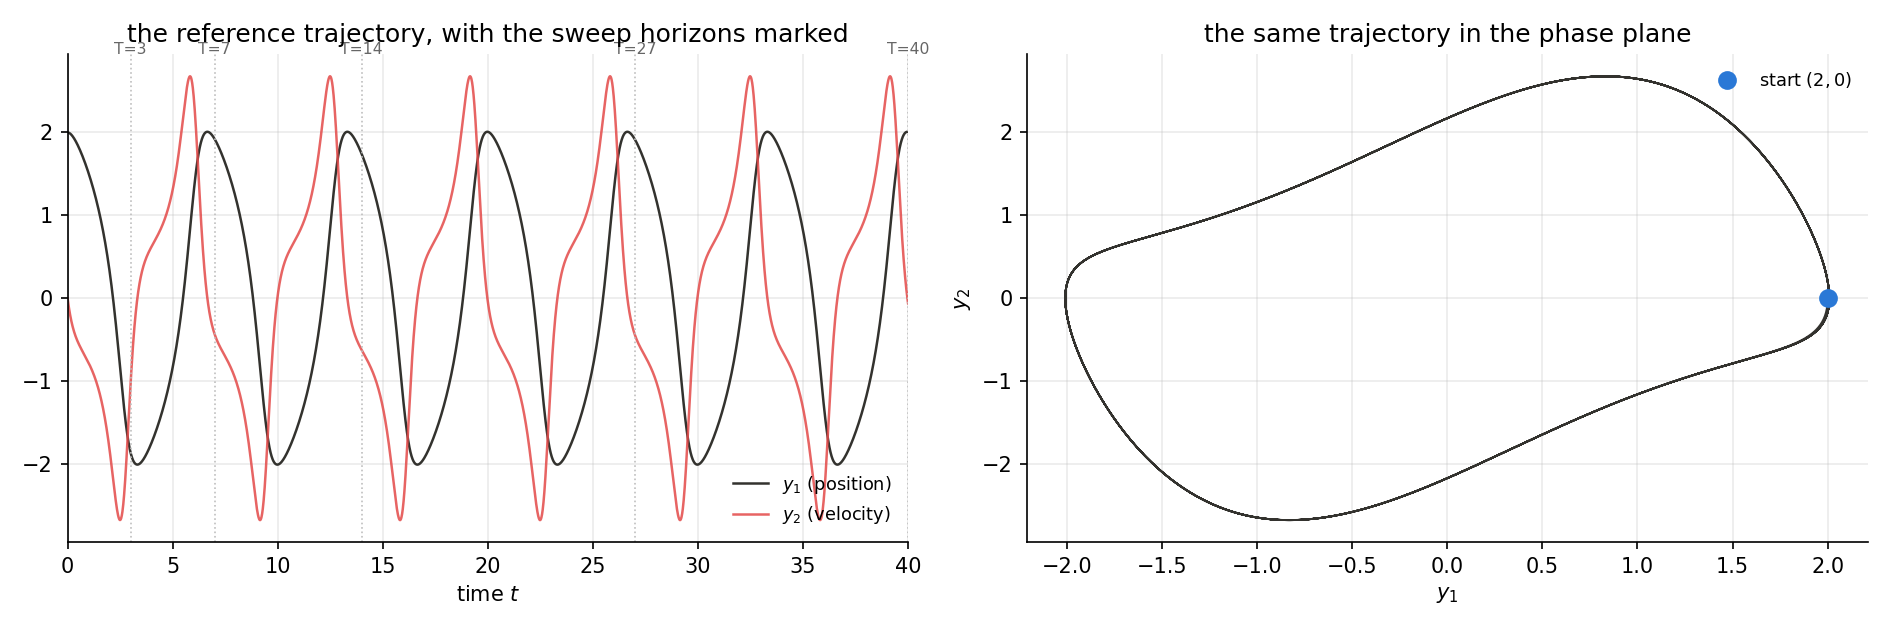
\includegraphics[width=\linewidth]{fig_problem.png}
  \caption{The test problem. Left: the reference trajectory from $(2,0)$
  over six periods, with the five training horizons of the continuous-time
  experiments marked. Right: the same trajectory in the phase plane, the
  closed loop to be learned.}
  \label{fig:problem}
\end{figure}

\subsection{The reference solution}

All errors are measured against a fixed-step, seven-stage, sixth-order
explicit Runge--Kutta integration of Eq.~\eqref{eq:vdp} at step
$10^{-3}$ in double precision, verified independently of any network by
four instruments, each measured rather than asserted:
\begin{enumerate}
  \item the convergence order, measured as the slope of the global error
  against the step size on logarithmic axes over three problems with known
  closed-form solutions (an order-$p$ method appears as slope $p$); the
  measured slopes are 6.06, 6.27 and 5.75 against the theoretical 6;
  \item step-halving self-consistency: integrating at $h$ and $h/2$ and
  comparing, the disagreement reaches a rounding floor of
  $6.4\times10^{-14}$ below $h \approx 5\times10^{-3}$, so at the working
  step $10^{-3}$ the truncation error is beneath double-precision
  rounding;
  \item the period of the limit cycle, $6.663287$ measured against the
  accepted value $6.6633$; and
  \item the closure of the limit cycle onto itself after one full period:
  $5.6\times10^{-14}$.
\end{enumerate}
The reference is trustworthy to approximately $10^{-13}$, six orders of
magnitude below anything a trained network reaches in this study, so the
yardstick never contaminates the measurement. The reference is used only
for scoring, never for training, with one deliberate exception: the
data-supervised baseline of Section~\ref{sec:baseline}, whose entire point
is to consume it. Where a network's evaluation times fall between stored
reference samples (the Gauss stage times of
Section~\ref{sec:disc-method}), the reference integrator is re-run to stop
exactly at each required time; nothing is interpolated.

\subsection{Error measures}
\label{sec:metrics}

I use three measures. Throughout the paper, whiskered quantities are
medians over random-initialisation seeds with whiskers spanning the
minimum to the maximum seed.
\begin{enumerate}
  \item \textbf{Relative $L_2$ error} (the headline number):
  $\varepsilon_{\mathrm{rel}} =
  \lVert y_\theta - y_{\mathrm{ref}} \rVert_2 /
  \lVert y_{\mathrm{ref}} \rVert_2$,
  with the norms taken over all evaluation times (or held-out states) and
  both components together; $y_\theta$ denotes the network output and
  $y_{\mathrm{ref}}$ the reference. Explicitly, for a trajectory sampled
  at times $\{t_k\}$,
  $\varepsilon_{\mathrm{rel}}^2 =
  \sum_k \lVert y_\theta(t_k) - y_{\mathrm{ref}}(t_k)\rVert^2 \big/
  \sum_k \lVert y_{\mathrm{ref}}(t_k)\rVert^2$.
  Read it as a fraction of the trajectory's overall size: $10^{-3}$ means
  the prediction differs from the truth by about a tenth of a percent of
  that size, and a value near 1 means the prediction is as wrong as the
  trajectory is large.
  \item \textbf{Scale-normalised pointwise error}:
  $|\hat y_i - y_i| / \max_t |y_{i,\mathrm{ref}}|$ per component, well
  defined even where a component crosses zero; used for error maps and
  curves.
  \item \textbf{Capped pointwise relative error}: the squared error
  normalised by the squared size of the true state and capped at one,
  \begin{equation}
    \rho \;=\; \min\!\left(1,\;
      \frac{\lVert y_{\mathrm{ref}} - y_\theta \rVert^2}
           {\lVert y_{\mathrm{ref}} \rVert^2}\right),
    \qquad
    \lVert y_{\mathrm{ref}} \rVert = \sqrt{y_{1,\mathrm{ref}}^2 + y_{2,\mathrm{ref}}^2},
    \label{eq:rho}
  \end{equation}
  evaluated per point (a time on a trajectory, or a held-out state). A
  worked example fixes the reading: for truth $(2, 0)$ and prediction
  $(1.9, 0.1)$ the error vector is $(0.1, -0.1)$, so
  $\rho = (0.1^2 + 0.1^2)/(2^2 + 0^2) = 0.02/4 = 0.005$; the prediction
  is wrong by half a percent of the state's squared size. The
  state-modulus denominator is deliberate: a
  componentwise denominator is undefined whenever that component crosses
  zero (twice per period for each component, and exactly at the start,
  where $y_2 = 0$), whereas the state modulus vanishes only at the
  equilibrium. The cap reads as ``one hundred percent wrong'' and engages
  only where the miss exceeds the state itself: on order-one failed fits,
  and at the single evaluation state of the discrete-time grid whose true
  image is exactly the origin. Two reporting rules follow. The
  \emph{median} of $\rho$ is robust and tracks fine structure; the
  \emph{mean} of $\rho$ (a mean squared error, since $\rho$ is already a
  squared quantity) over the discrete-time evaluation grid of 441 states
  carries a fixed $1/441 \approx 2.3\times10^{-3}$ contribution from the
  one capped origin state and cannot resolve anything below it, so it is
  quoted only together with its cap count. Because $\rho$ is squared,
  $\sqrt{\rho}$ compares directly with relative $L_2$ values, and the two
  metrics cross-check each other throughout (for example, the selected
  network of Section~\ref{sec:disc-size} has six-period
  $\rho = 2.0\times10^{-6}$, i.e.\
  $\sqrt{\rho} \approx 1.4\times10^{-3}$, consistent with its
  independently computed chained relative $L_2$ of $2.0\times10^{-3}$).
\end{enumerate}

% ===========================================================================
\section{The continuous-time formulation}
\label{sec:cont-method}

\subsection{Method}

The source work considers equations $u_t + \mathcal{N}[u] = 0$, defines the
residual $f := u_t + \mathcal{N}[u]$, approximates $u$ by a network, and
obtains the residual of the network by automatic differentiation, the
exact, chain-rule differentiation of the network with respect to its own
inputs. The loss is the equally weighted sum of two mean-squared terms: a
data term over the $N_u$ points where the solution is known (initial and
boundary data), and a residual term over $N_f$ sampled \emph{collocation
points}, the classical term for locations at which an equation is enforced.

For an ordinary differential equation the transfer is direct, with three
simplifications and one declared deviation. There is no spatial coordinate:
the network maps one input, time, to the two-component state
$y_\theta(t)$. There is no boundary: the data term collapses to a single
anchor, the requirement that the network at $t = 0$ equal the starting
state. This is one anchored point in place of the 50--100 used by the
source work's demonstrations, which makes the anchor's task
correspondingly harder. No spatial derivatives survive either: the only
differentiation left is the time derivative of the network,
$\dot y_\theta(t)$, obtained by differentiating the network's output with
respect to its own input. Automatic differentiation therefore appears in
two distinct roles that should not be conflated: derivatives of the loss
with respect to the weights $\theta$ drive the optimiser, as in any
network training, while derivatives of the network output with respect to
its input $t$ build the residual itself. Both are exact chain-rule
computations, with no finite differences anywhere. The residual and loss
are the exact transcription of the source construction,
\begin{equation}
  r(t) = \begin{pmatrix}
    \dot y_{1,\theta}(t) - y_{2,\theta}(t) \\[2pt]
    \dot y_{2,\theta}(t) - \mu\big(1 - y_{1,\theta}^2(t)\big)\,
      y_{2,\theta}(t) + y_{1,\theta}(t)
  \end{pmatrix},
  \qquad
  \mathcal{L} = \big\lVert y_\theta(0) - y^0 \big\rVert^2
  + \frac{1}{N}\sum_{i=1}^{N} \big\lVert r(t_i) \big\rVert^2 ,
  \label{eq:contloss}
\end{equation}
with $y^0 = (2,0)$ and $\{t_i\}$ the collocation times. The one deviation:
time is affinely mapped to $[-1,1]$ inside the network, because
hyperbolic-tangent layers condition badly on raw inputs of size 40; this is
declared so that the failure that remains is honestly the method's rather
than a units artefact. The formulation also inherits a structural
limitation from the source work: the starting state enters through the loss
and is baked into the trained weights, so each trained network serves
exactly one initial condition.\footnote{An expensive way to solve one
initial-value problem, and an equally expensive way to solve each
subsequent one.} The discrete-time formulation of
Section~\ref{sec:disc-method} removes exactly this.

\subsection{Collocation budget}
\label{sec:collocation}

Because the collocation budget is central to how the source work frames the
limitations of this formulation, I fix it explicitly and generously. The
density is 20 collocation points per unit time at every horizon, placed by
one-dimensional Latin hypercube sampling (a stratified random design: one
point per equal-width stratum, so the domain is covered without
clustering). A longer horizon therefore receives proportionally more
points and is never undersampled by construction:
$N = 60,\ 140,\ 280,\ 540,\ 800$ collocation points at the five horizons of
Table~\ref{tab:expA}. For comparison, the source work's continuous-time
demonstrations use $20{,}000$ collocation points (Schr\"odinger equation)
and $10{,}000$ (Burgers equation) over two-dimensional space--time domains.
On this problem the entire budget costs fractions of a second to evaluate;
every experiment below pays it in full. Whatever fails in
Section~\ref{sec:cont-results} therefore does not fail for want of
collocation points. Sections~\ref{sec:density} and~\ref{sec:placement}
then vary the density over a 64-fold range and the placement directly,
closing the collocation axis by measurement.

\subsection{Protocol}
\label{sec:cont-protocol}

All continuous-time experiments share: a fully connected network of 4
hidden layers of 50 hyperbolic-tangent units, in double precision (until
Section~\ref{sec:size-start} varies the architecture). Written out, the
network computes
\begin{equation*}
  h_1 = \tanh(W_1 t + b_1), \quad
  h_k = \tanh(W_k h_{k-1} + b_k) \;\; (k = 2, \dots, 4), \quad
  y_\theta(t) = W_5 h_4 + b_5 ,
\end{equation*}
with the weight matrices and bias vectors $W_k, b_k$ collectively
denoted $\theta$. The hyperbolic tangent is used because it is smooth
everywhere, and smoothness matters here: the residual of
Eq.~\eqref{eq:contloss} differentiates the network, so a kinked
activation such as the rectifier would hand the residual a discontinuous
derivative. Training horizons are
$T \in \{3, 7, 14, 27, 40\}$, i.e.\ 0.45 to 6.0 periods of the limit
cycle (dividing by the period $6.663287$), bracketing one period from
either side, with three
random-initialisation seeds per horizon, so that a single initialisation
cannot masquerade as the method's verdict.\footnote{A seed fixes the
random initial weights and nothing else; a run is otherwise deterministic,
so every number in this paper reproduces bit for bit.} The optimiser is
full-batch L-BFGS (a deterministic quasi-Newton method using the entire
loss at every step, as in the source work) with strong Wolfe line search,
up to 6 restarts of 200 iterations, stopping early after two consecutive
restarts improve the loss by less than 1\%. This is a convergence
criterion rather than a budget, so every plain-formulation failure below
is a converged failure. Scoring is on the dense reference grid (spacing
$0.01$) with the measures of Section~\ref{sec:metrics}.

\subsection{Results: faithful reproduction}
\label{sec:cont-results}

\begin{table}[tbp]
  \centering
  \caption{Faithful reproduction of the continuous-time formulation, swept
  over the training horizon. $N$ is the number of collocation points
  (density fixed at 20 per unit time). Median, best and worst are over
  three seeds; the loss is the converged training loss.}
  \label{tab:expA}
  \small
  \begin{tabular}{cccccc}
    \toprule
    $T$ & periods & $N$ & rel.\ $L_2$ (median) & best / worst seed & final loss \\
    \midrule
    3  & 0.45 & 60  & $3.8\times10^{-5}$ & $2.3\times10^{-5}$ / $4.6\times10^{-5}$ & $1.4$--$2.0\times10^{-7}$ \\
    7  & 1.05 & 140 & $6.6\times10^{-4}$ & $4.8\times10^{-4}$ / $3.9\times10^{-3}$ & $2.3\times10^{-6}$--$2.8\times10^{-5}$ \\
    14 & 2.10 & 280 & $0.79$             & $0.789$ / $0.805$                       & $\approx 6\times10^{-2}$ \\
    27 & 4.05 & 540 & $0.90$             & $0.903$ / $0.905$                       & $\approx 3\times10^{-2}$ \\
    40 & 6.00 & 800 & $0.94$             & $0.936$ / $2.09$                        & $2.1$--$4.8\times10^{-2}$ \\
    \bottomrule
  \end{tabular}
\end{table}

Table~\ref{tab:expA} and Figure~\ref{fig:cliff} give the central result of
the reproduction. Below one period the formulation is excellent: at
$T = 3$ the median relative $L_2$ error is $3.8\times10^{-5}$, at or better
than the accuracy the source work reports for its own continuous-time
demonstrations ($1.97\times10^{-3}$ for the Schr\"odinger equation,
$6.7\times10^{-4}$ for the Burgers equation). This is unsurprising for a
two-state oscillator against partial differential equations, but it
confirms that the machinery is correctly built. Beyond one period the
error is of order one at every horizon and every seed, with the seeds
agreeing to two decimal places: the failure is systematic, not
initialisation luck.

\begin{figure}[tbp]
  \centering
  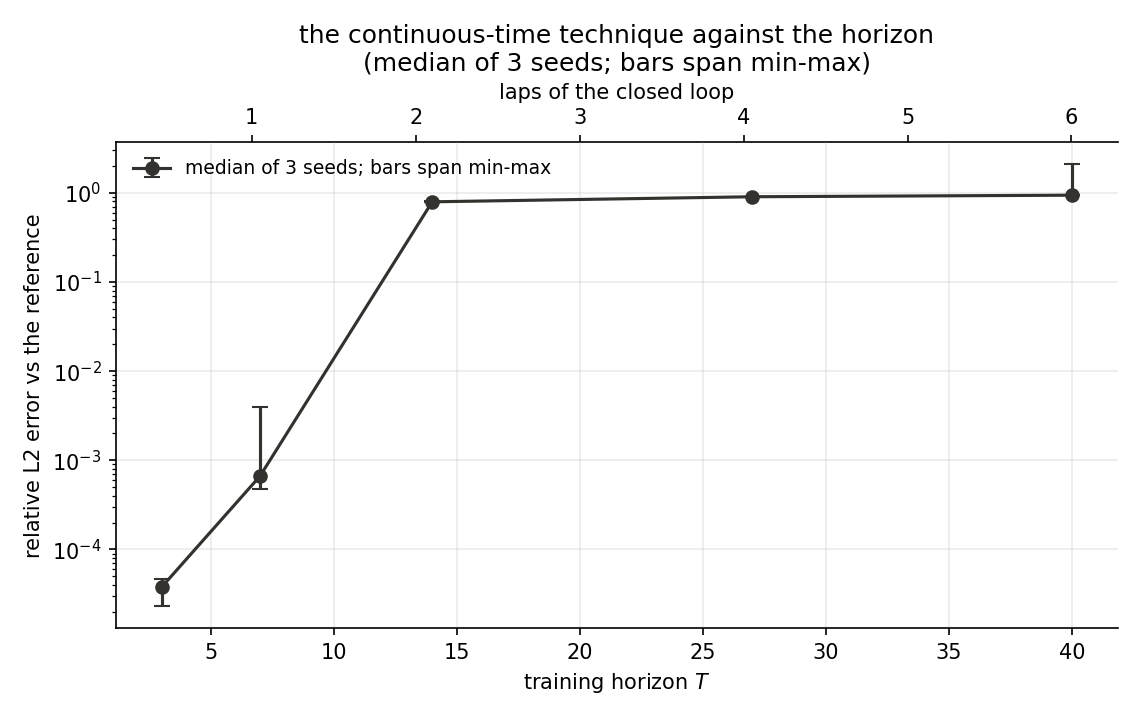
\includegraphics[width=0.72\linewidth]{fig_cliff.png}
  \caption{Relative $L_2$ error against training horizon for the faithful
  reproduction; median of three seeds with min--max whiskers. The
  formulation is excellent below one period of the limit cycle and fails
  at order unity beyond it.}
  \label{fig:cliff}
\end{figure}

\begin{figure}[tbp]
  \centering
  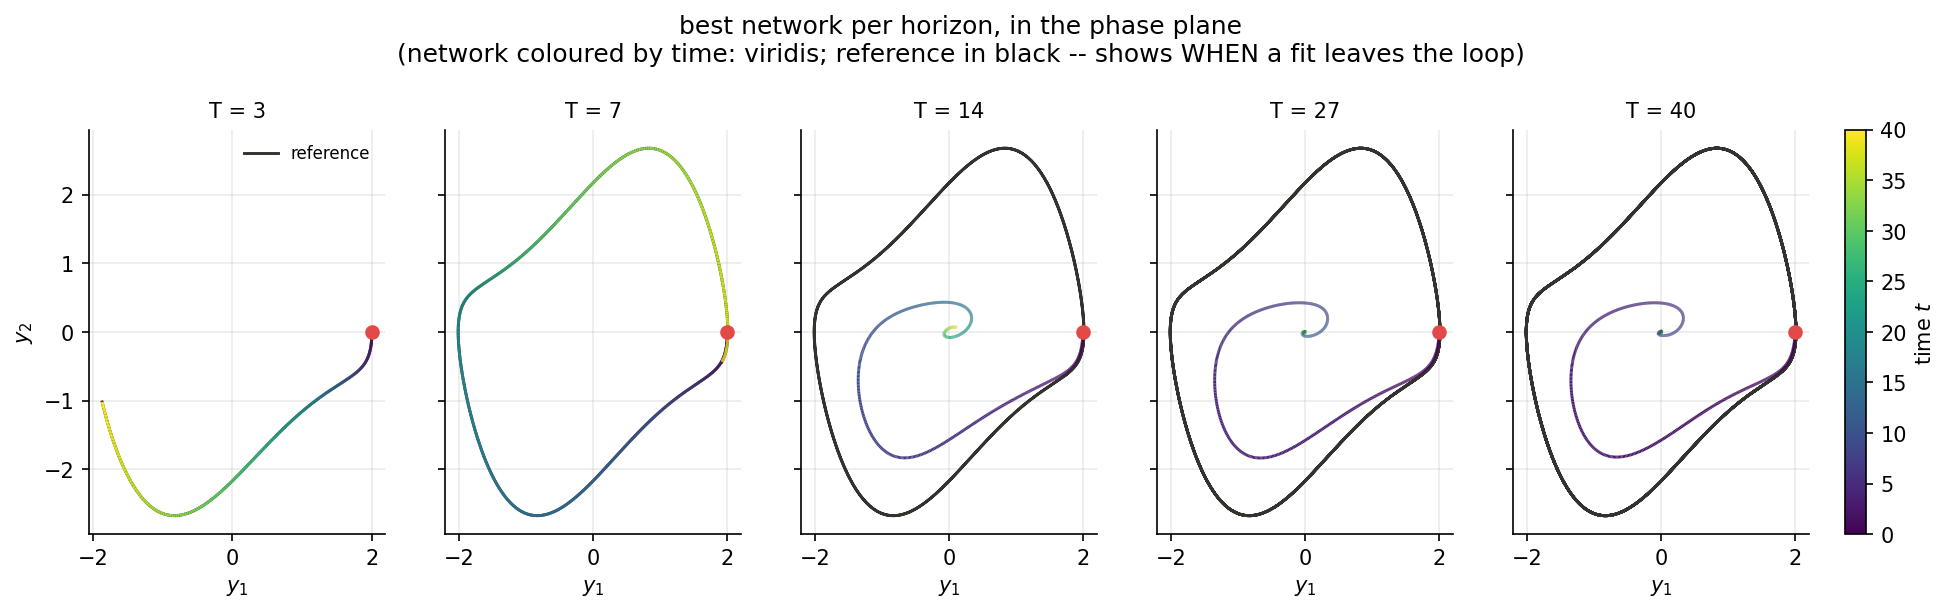
\includegraphics[width=\linewidth]{fig_phase_collapse.png}
  \caption{The failed fits in the phase plane (best seed per horizon).
  Past the one-period boundary the fit abandons the closed loop and spirals
  into the origin, the repelling equilibrium, against the direction of the
  true flow.}
  \label{fig:phase-collapse}
\end{figure}

\begin{figure}[tbp]
  \centering
  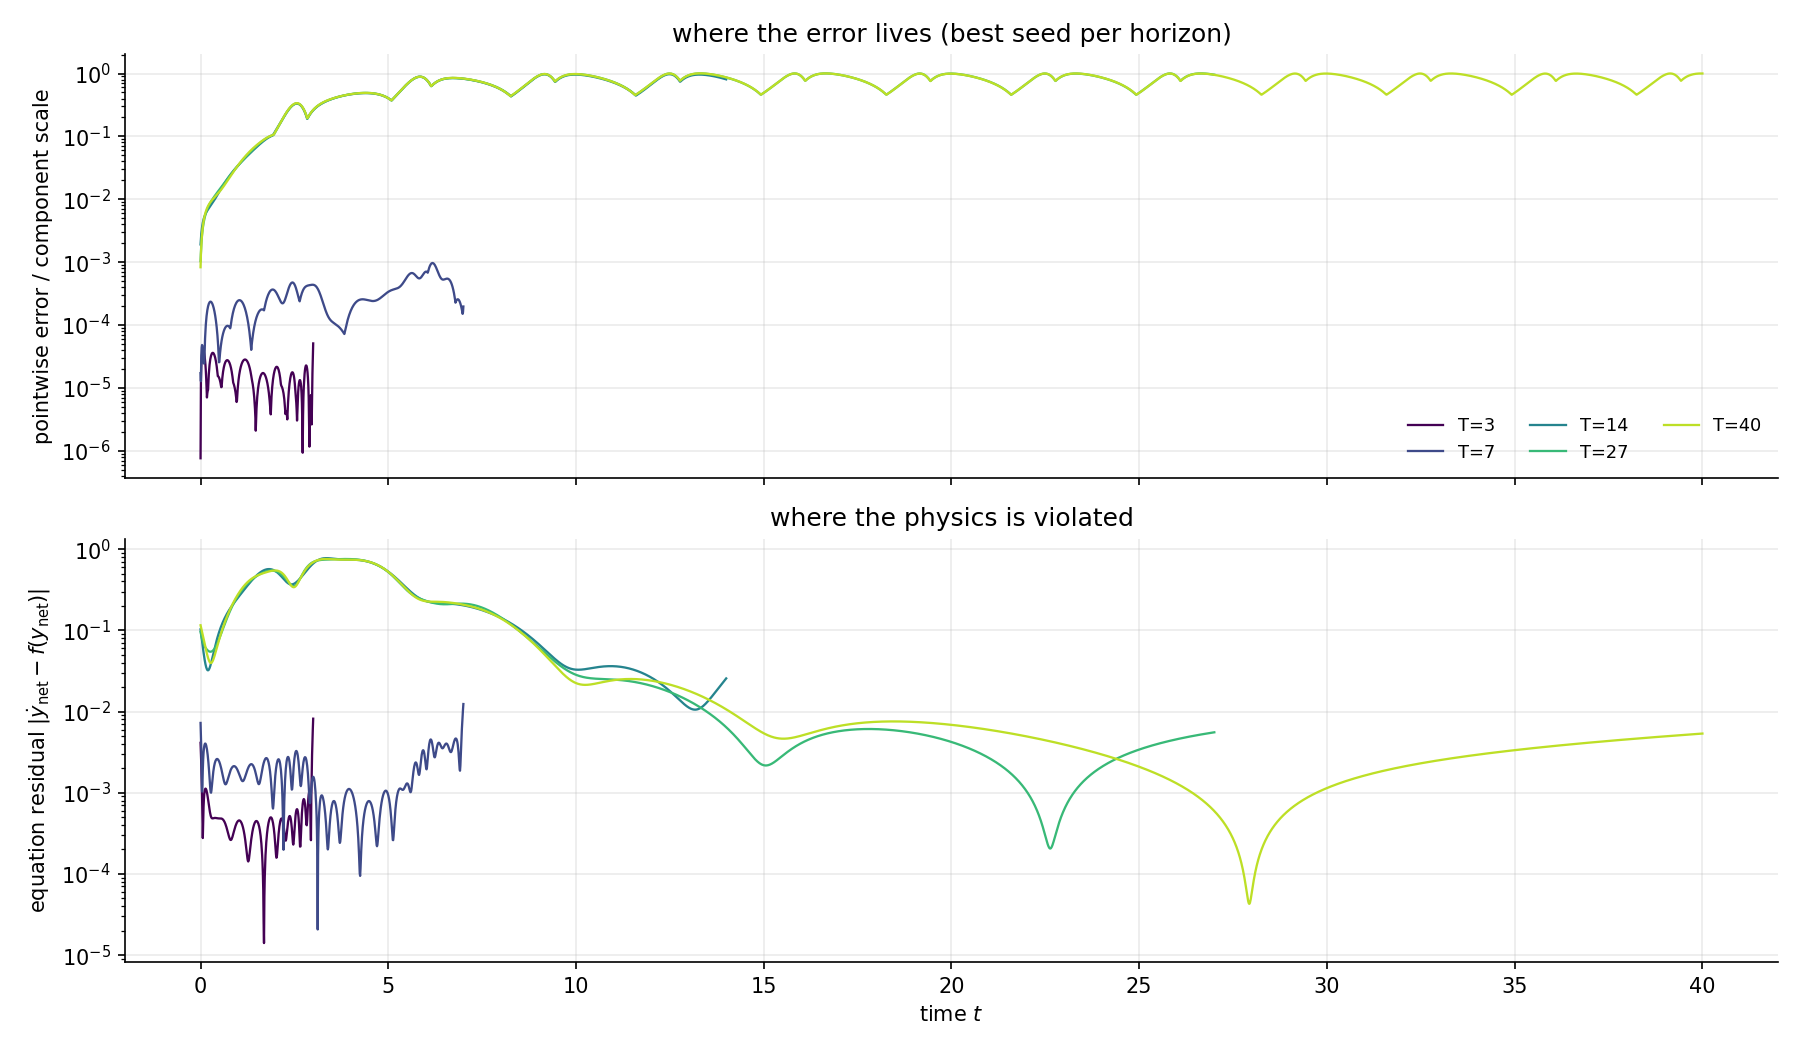
\includegraphics[width=\linewidth]{fig_diagnosis.png}
  \caption{The failure mechanism. Top: where the error lives in time
  (logarithmic scale). Bottom: the equation residual along the network's
  own trajectory. Past the failure boundary the residual is paid only in a
  short escape window and is negligible ever after: the physics is
  satisfied, on the wrong solution.}
  \label{fig:diagnosis}
\end{figure}

The mechanism is visible in Figures~\ref{fig:phase-collapse}
and~\ref{fig:diagnosis}. The origin satisfies Eq.~\eqref{eq:vdp} exactly,
so a network that parks there pays no residual at all. The true dynamics
repel from the origin, but a pointwise residual contains no stability
information, so the loss cannot distinguish the attracting truth from the
repelling impostor. The residual cost of escaping the true trajectory is
confined to a short window of fixed size, and the mean over collocation
points divides that fixed cost by the horizon, so the impostor becomes
cheaper as $T$ grows. At $T = 3$ the escape would corrupt most of the
domain and the truth wins; at $T = 14$ it costs one period out of two and
every seed falls. One $T = 40$ seed found a more ambitious escape, the
$2.09$ outlier in Table~\ref{tab:expA}.\footnote{Instead of parking at the
origin it drifted outward to $y_1 \approx 4.7$, well outside the loop, and
settled on a different wrong curve: the same mechanism with a different
destination.}

Two conclusions follow. First, the failure is silent: the final losses
converge to values of order $10^{-2}$ (Table~\ref{tab:expA}) while the
error is of order one, so a small, converged training loss is not evidence
of a correct solution. Second, the failure is a measured counterexample to
the source work's general claim that, for a well-posed problem with a
unique solution, good accuracy follows from a sufficiently expressive
network and sufficiently many collocation points. The problem here is
well-posed with a unique solution, the identical network fits $T = 7$, and
the collocation budget is trivially affordable and fully paid
(Section~\ref{sec:collocation}), yet the method returns the wrong solution
with a converged loss. What the loss lacks is anchoring: information about
which solution is wanted, spread across the domain instead of concentrated
at a single point. Collocation coverage is not the missing ingredient.

\subsection{Causal weighting and its limits}
\label{sec:causal}

\subsubsection{Method}

The diagnosis above is that the loss fits all times simultaneously: late
times settle onto a spurious solution before any information from the
single anchor at $t = 0$ can reach them, because nothing in
Eq.~\eqref{eq:contloss} encodes that an initial-value problem is determined
forward in time. Causal weighting~\cite{wang2024causal} encodes exactly
that and nothing else. The residual at collocation time $t_i$ is weighted
by
\begin{equation}
  w_i = \exp\!\Big(-\varepsilon \int_0^{t_i} |r(s)|^2 \, ds\Big),
  \label{eq:causal}
\end{equation}
with the integral evaluated as a left Riemann sum over the sorted
collocation times $t_{(1)} < t_{(2)} < \dots$: writing
$\Delta t_{(j)} = t_{(j)} - t_{(j-1)}$,
\begin{equation*}
  \int_0^{t_i} |r(s)|^2 \, ds \;\approx\;
  \sum_{j\,:\,t_{(j)} < t_i} \big\lVert r(t_{(j)}) \big\rVert^2\,
  \Delta t_{(j)} .
\end{equation*}
The time-weighting of the sum is deliberate: because $\varepsilon$
multiplies a time-integral rather than a bare sum over points, its
meaning is independent of collocation density and horizon, and doubling
the number of points does not double the exponent. The weights are
recomputed from the current residuals at every optimiser iteration but
treated as fixed constants by the gradient (detached from the
differentiation), so the optimiser never gains by manipulating its own
weighting. A collocation
point counts only once the trajectory \emph{before} it already satisfies
the equation: a front of solved trajectory propagates outward from the
anchor, and the far domain cannot be captured by an impostor while its
weights are still negligible. On convergence all residuals vanish, every
weight rises to 1, and the objective becomes exactly the unweighted loss,
so the weighting is temporary scaffolding that is gone by the end of a
successful training.

The weighting is incompatible with L-BFGS, which requires a stationary
objective; I measured two hybrid schedules, and both fail:
\begin{itemize}
  \item freezing the weights per L-BFGS restart lets the front advance
  only at the six refreezes; it stalled 42\% of the way across $T = 14$
  (relative error $2.15$);
  \item splitting the same 1200 iterations into 40 short restarts starves
  each restart instead; the front oscillated around 30\% (relative error
  $1.58$).
\end{itemize}
The front must move continuously; per-iteration weight updates are part of
the method. The algorithm actually used therefore follows the
causal-weighting authors:
\begin{enumerate}
  \item an Adam phase (learning rate $10^{-3}$), with the weights
  recomputed from detached residuals at every iteration;
  \item $\varepsilon$ annealed upward through the ladder
  $\{0.01, 0.1, 1, 10, 100\}$ (small $\varepsilon$ tolerates upstream
  error; large $\varepsilon$ demands it be gone), advancing one rung
  whenever the smallest weight exceeds $0.99$, all within a budget of
  $60{,}000$ Adam steps; and
  \item the identical L-BFGS polish of Section~\ref{sec:cont-protocol} on
  the plain unweighted loss, once every weight is near 1.
\end{enumerate}
Causal weighting thus acts as a warm start that delivers L-BFGS into the
right basin, and both sides of the comparison end by optimising the same
objective with the same optimiser. Two quantities are logged throughout as
telemetry: the minimum weight, and the fraction of collocation points with
weight above one half, the ``awake fraction''.\footnote{A collocation
point with weight above one half is awake, and the far domain, weights
near zero, is asleep. The names are informal but the telemetry is not.}

\subsubsection{Results}

\begin{table}[tbp]
  \centering
  \caption{Unweighted versus causally weighted training at equal collocation
  density, architecture and budget. Medians over three seeds.}
  \label{tab:causal}
  \small
  \begin{tabular}{ccccl}
    \toprule
    $T$ & periods & unweighted & causal & front status (steps to arrive) \\
    \midrule
    3  & 0.45 & $3.8\times10^{-5}$ & $4.8\times10^{-5}$ & arrived, 3--5.5k \\
    7  & 1.05 & $6.6\times10^{-4}$ & $7.6\times10^{-5}$ & arrived, 8.5--28.5k \\
    14 & 2.10 & $0.79$             & $2.1\times10^{-4}$ & capped; 2 of 3 seeds crossed, third starved ($0.71$) \\
    27 & 4.05 & $0.90$             & $1.90$             & capped mid-crossing, all seeds ($0.88$/$1.90$/$1.99$) \\
    40 & 6.00 & $0.94$             & $2.04$             & capped mid-crossing, all seeds ($0.95$/$2.04$/$2.27$) \\
    \bottomrule
  \end{tabular}
\end{table}

\begin{figure}[tbp]
  \centering
  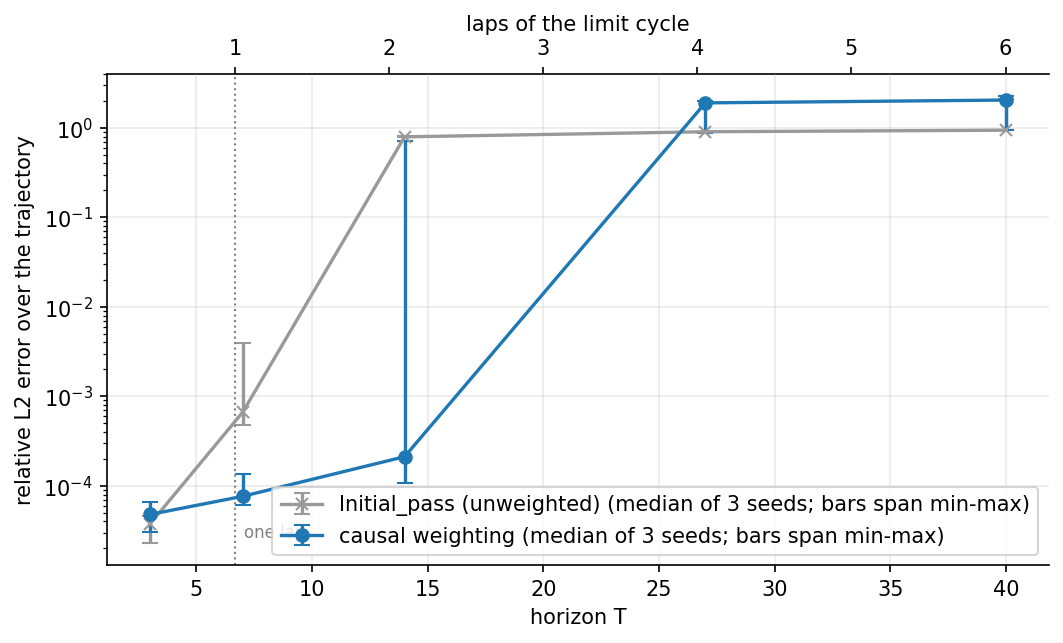
\includegraphics[width=0.8\linewidth]{fig_causal_compare.png}
  \caption{Same metric, reference, collocation density and budget on both
  sides; only the weighting differs. Median of three seeds with min--max
  whiskers. Causal weighting moves the failure boundary from between one
  and two periods to between two and four.}
  \label{fig:causal-compare}
\end{figure}

\begin{figure}[tbp]
  \centering
  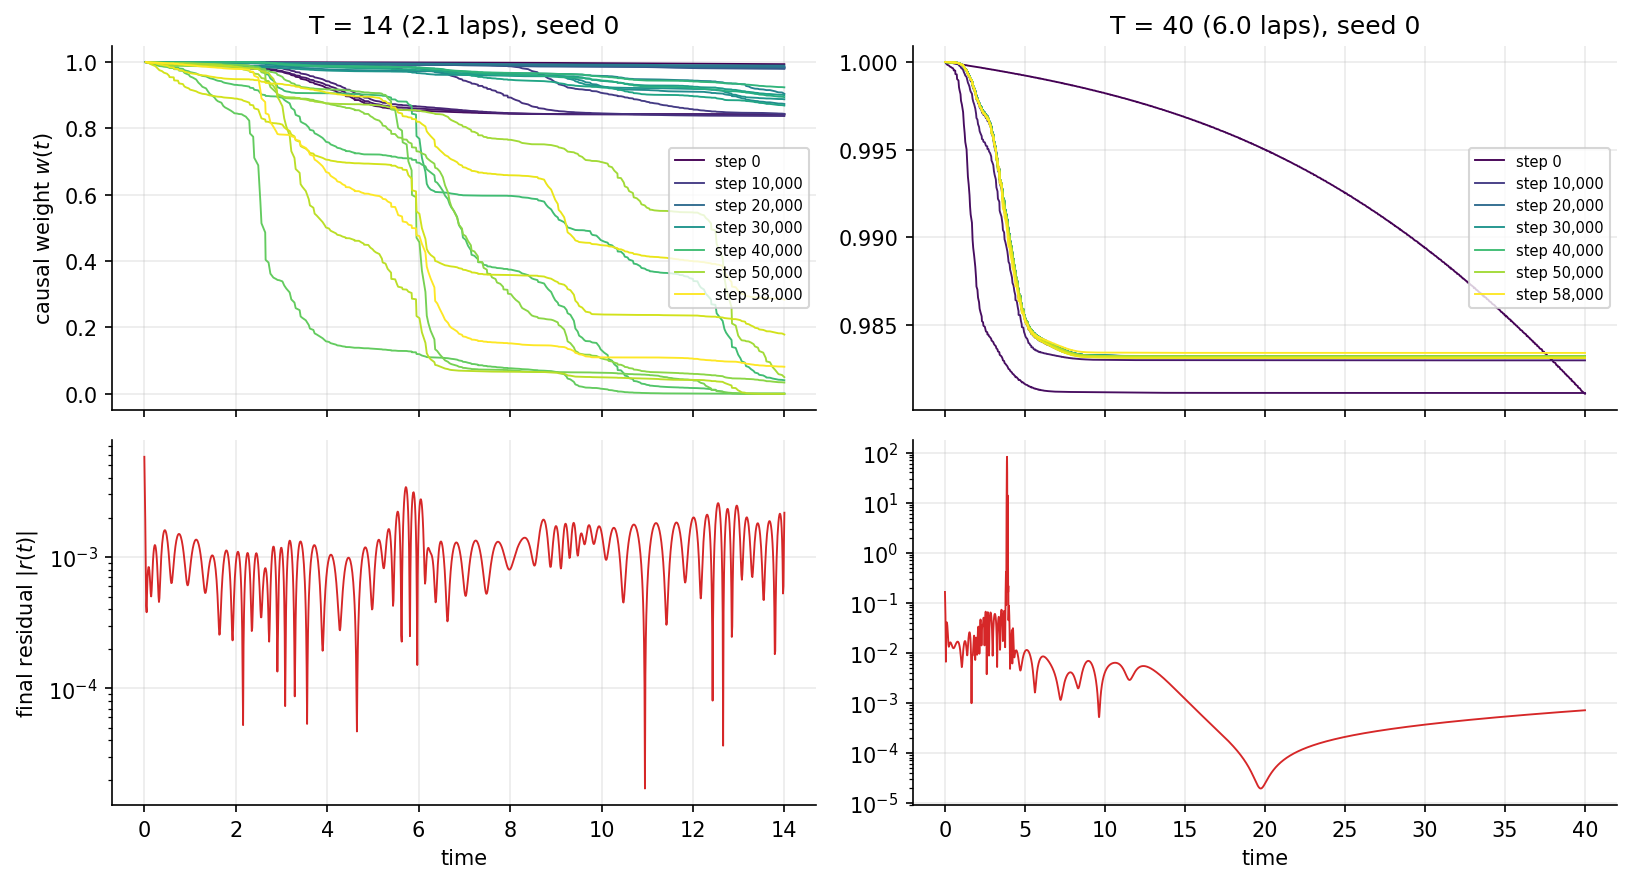
\includegraphics[width=\linewidth]{fig_causal_front.png}
  \caption{The mechanism at work: snapshots of the weight profile $w(t)$
  during training (colour: optimiser step) at $T=14$ and $T=40$; below,
  the equation residual along the final fit. A front of awake collocation
  points sweeps outward from the anchor as the trajectory behind it becomes
  consistent with the equation.}
  \label{fig:causal-front}
\end{figure}

Table~\ref{tab:causal} and Figure~\ref{fig:causal-compare} summarise the
comparison. At $T = 14$ (two periods, where the unweighted formulation
fails at $0.79$) causal weighting reaches $2.1\times10^{-4}$, an
improvement of three to four orders of magnitude; in the capped metric of
Eq.~\eqref{eq:rho} the contrast at $T=14$ is about seven orders of
magnitude. The cost of crossing the domain grows faster than linearly:
roughly $3.5$k optimiser steps at half a period, $10$--$30$k at one
period, $60$k at two, and beyond the budget at four and six periods,
where runs caught mid-crossing score \emph{worse} than the unweighted
baseline because the still-asleep tail of the domain is unconstrained.
The essential difference from Section~\ref{sec:cont-results} is that
these failures are flagged: the telemetry reads ``still crossing''. The
unweighted failures, by contrast, reported themselves as converged. One
starved seed also produced the study's second loophole: a fit with
training loss $9.7\times10^{-6}$ and error $0.71$, an out-of-phase
near-solution joined to the truth by a jump \emph{between} collocation
points, invisible both to the loss and to weights computed on the same
grid. Sections~\ref{sec:density} and~\ref{sec:placement} test directly
whether more points, or better-placed points, close these loopholes.

\subsubsection{The budget-extension test}

Every causally weighted run at $T \ge 14$ ended at the $60$k-step cap with
its front mid-crossing. So is the long-horizon failure simply budget
starvation? The test is direct: rerun exactly those seven runs at
$240{,}000$ steps, four times the budget, with nothing else changed.

\begin{table}[tbp]
  \centering
  \caption{The budget-extension test: the seven capped runs rerun at four
  times the optimisation budget. Zero of seven crossed.}
  \label{tab:extended}
  \footnotesize
  \begin{tabular}{lccl}
    \toprule
    run & 60k steps & 240k steps & telemetry reading \\
    \midrule
    $T=14$, seed 2 & 0.71 & 0.61 & certified arrival at 92k steps, still wrong (between-point jump) \\
    $T=27$, seed 0 & 0.88 & 0.83 & still crossing; advance far slower than linear in steps \\
    $T=27$, seed 1 & 1.90 & 0.24 & entrenched ${\sim}185$k steps; the gain tracked the annealing advance \\
    $T=27$, seed 2 & 1.99 & 1.99 & stuck at the gate; awake fraction below 0.1 throughout \\
    $T=40$, seed 0 & 0.95 & 0.79 & still crossing \\
    $T=40$, seed 1 & 2.04 & 2.08 & entrenched, weakly causal for the whole run \\
    $T=40$, seed 2 & 2.27 & 2.29 & stuck at the gate for the whole run \\
    \bottomrule
  \end{tabular}
\end{table}

\begin{figure}[tbp]
  \centering
  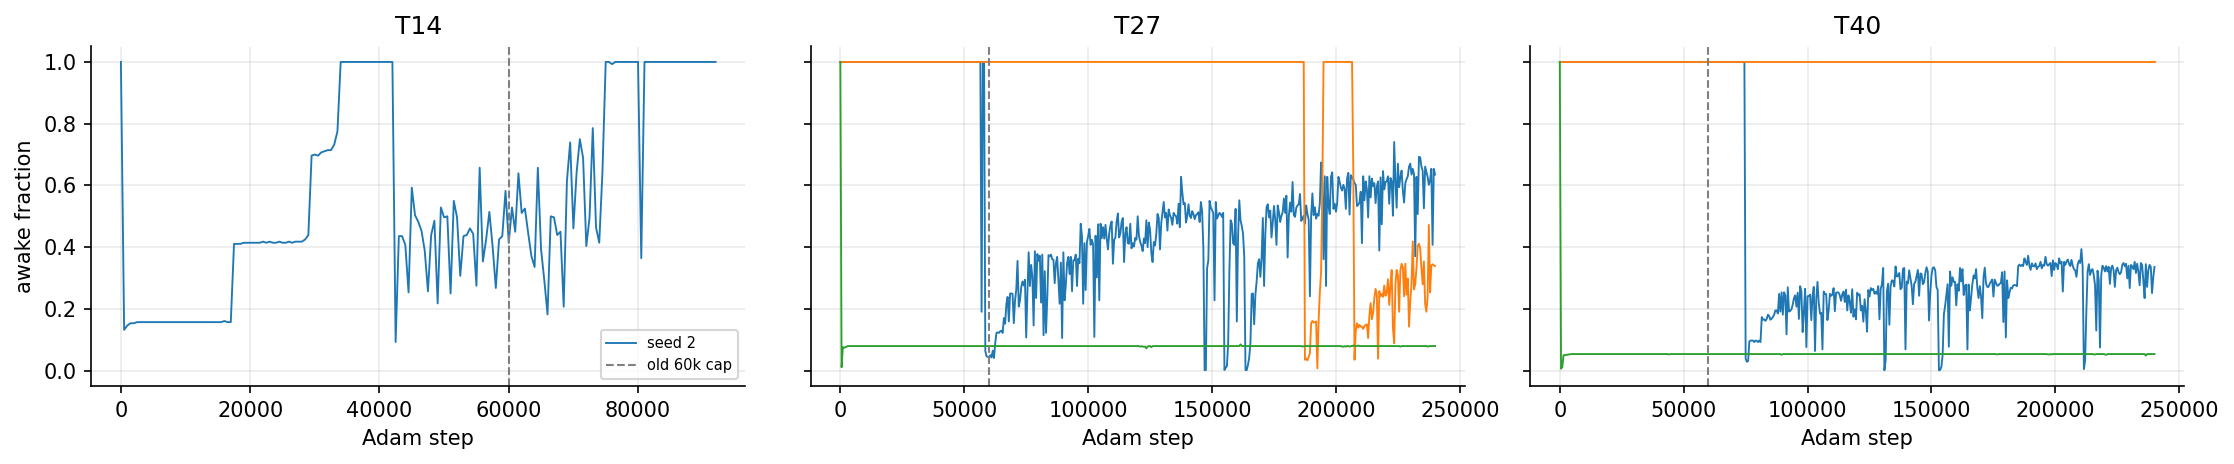
\includegraphics[width=\linewidth]{fig_telemetry.png}
  \caption{The discriminating instrument: the awake fraction over the
  extended runs, with the original 60k cap marked. The three failure modes
  are directly visible: the slow grind, the saturated-but-stuck plateau
  (note the $T=27$ transition near 185k steps, where the annealing finally
  advances and progress begins), and the flatline near zero.}
  \label{fig:telemetry}
\end{figure}

\begin{figure}[tbp]
  \centering
  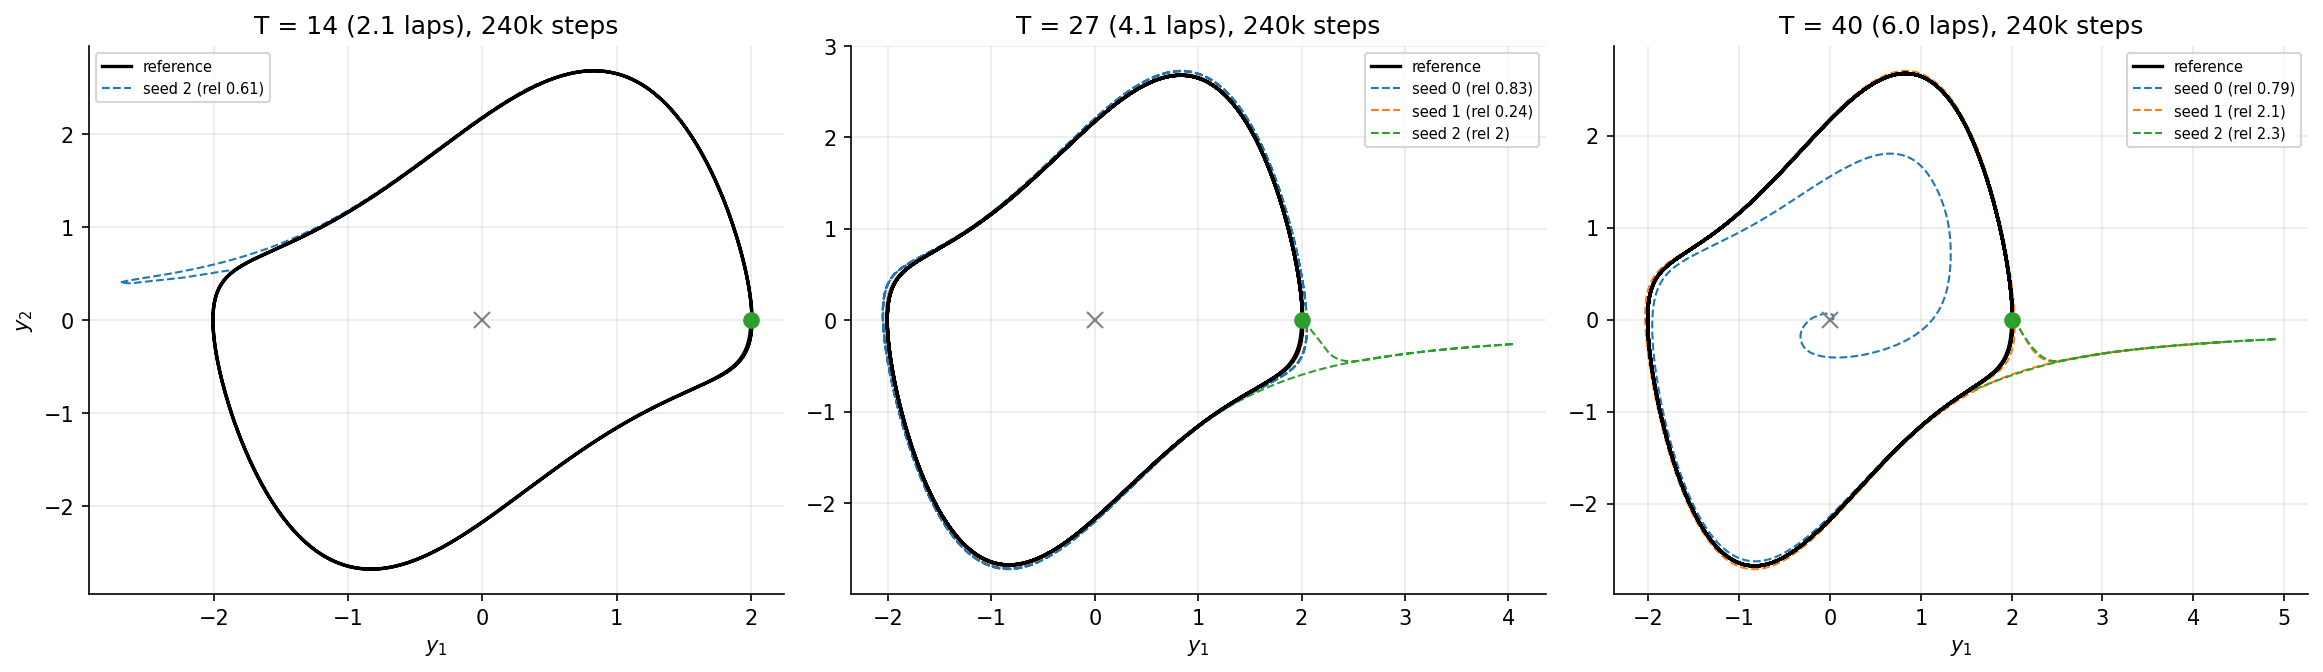
\includegraphics[width=\linewidth]{fig_extended_phase.png}
  \caption{Every extended-budget run in the phase plane. The entrenched
  seeds ride the reference loop almost perfectly and are wrong \emph{in
  time}: circulation out of phase, trajectory error of order one while the
  orbit looks flawless. The stuck-at-the-gate seeds satisfy the anchor and
  then jump off the loop. The one certified arrival traces the loop with a
  single excursion, the between-point escape that survived
  certification.}
  \label{fig:extended-phase}
\end{figure}

Table~\ref{tab:extended} answers the question: the original cap did
genuinely starve some seeds (one front needed 92k steps to arrive), but
four times the budget crossed zero of seven runs. The telemetry
(Figure~\ref{fig:telemetry}) separates three failure modes, and the phase
portraits (Figure~\ref{fig:extended-phase}) show what each looks like as a
trajectory. In the first, \emph{still crossing}, the front advances but
too slowly to finish. In the second, \emph{stuck at the gate}, the
annealing-advance criterion is never met even at the first $\varepsilon$
rung, so no front ever forms. In the third, \emph{entrenched}, the
weights saturate while $\varepsilon$ is still small, so training is
effectively unweighted and cements an impostor; the one entrenched seed
that eventually advanced, $T=27$ seed 1, improved to $0.24$, which is
still an order-one failure, and the improvement tracked the annealing
advance rather than the added steps. The binding constraints are
structural: (i) the annealing dynamics, since the whole-history integral
in Eq.~\eqref{eq:causal} tightens the wake-up criterion as the horizon
grows and the schedule can strand a run either asleep or weakly causal;
and (ii) the discretisation hole, since both the loss and the weights
see only the collocation grid, so a jump between grid points defeats even
a certified front arrival. Neither constraint yields to optimisation
budget at fixed collocation density.

\subsection{Network size and the starting state}
\label{sec:size-start}

The budget axis being closed, the next candidate resource is the network
itself, and with it a variable every experiment so far had frozen: the
starting state. I cross depth $\{2,4,6,8,10\}$ with width
$\{16,32,64,128,256\}$ (25 architectures), with both training arms
(plain, causally weighted), two horizons ($T=14$, the plain arm's first
collapse; $T=27$, the causal arm's first starvation), and six starting
states: $(2,0)$ plus five Latin-hypercube-drawn states across the
rectangle $y_1 \in [-2.5, 2.5]$, $y_2 \in [-3, 3]$ (the limit cycle with
margin, and the same region the discrete-time formulation later trains
over), one seed each: $25 \times 2 \times 2 \times 6 = 600$ runs, and
$25 \times 6 = 150$ runs per (arm, horizon) cell.

No architecture rescues a failing horizon
(Figure~\ref{fig:size-heatmaps}). In the plain arm at $T=14$ every
architecture fails, with per-cell medians over the six starts of
0.82--0.99 and a best single run of 0.272 across all 150; at $T=27$ the
medians are 0.93--0.98. In the causal arm at $T=14$ there is no monotonic
improvement with size (best cell: depth 2, width 64, median 0.151; most
cells 0.4--1.2), and at $T=27$ the wall is flat: cell medians 0.86--1.22
and a best single run of 0.685. Nothing succeeds at four periods, at any
size. Two structural readings hold across arms and horizons: added depth
is actively harmful, and added width saturates by 64--128 units.

\begin{figure}[tbp]
  \centering
  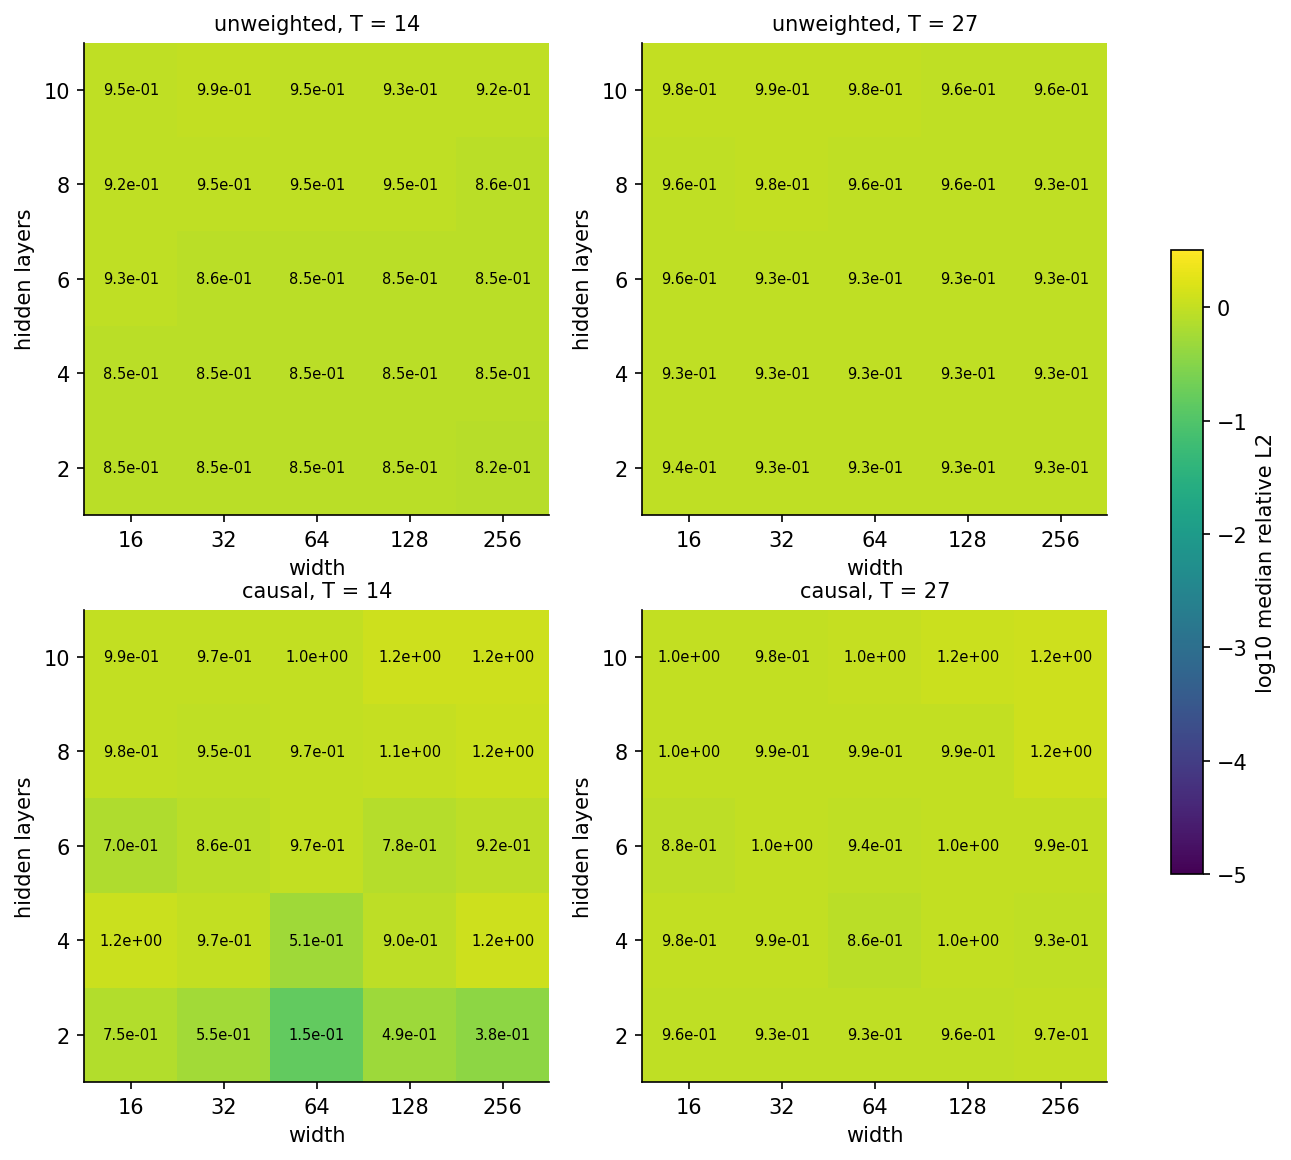
\includegraphics[width=\linewidth]{fig_size_heatmaps.png}
  \caption{Median relative $L_2$ error by architecture (depth $\times$
  width), one heatmap per training arm and horizon, medians over the six
  starting states: no row or column rescues the failing horizons.
  Network size does not move the wall.}
  \label{fig:size-heatmaps}
\end{figure}

\begin{table}[tbp]
  \centering
  \caption{Success by starting state: causally weighted arm at $T=14$ (two
  periods), counting a run a success at relative $L_2 < 10^{-2}$, out of
  the 25 architectures per start. $\lVert y^0 \rVert$ is the start's
  distance from the repelling equilibrium at the origin.}
  \label{tab:starts}
  \small
  \begin{tabular}{cccc}
    \toprule
    start $(y_1, y_2)$ & $\lVert y^0 \rVert$ & successes / 25 & best run \\
    \midrule
    $(2.00, 0.00)$   & 2.00 & 9 & $6.7\times10^{-5}$ \\
    $(1.85, 2.90)$   & 3.45 & 6 & $1.1\times10^{-3}$ \\
    $(-2.32, -2.79)$ & 3.63 & 3 & $1.5\times10^{-3}$ \\
    $(0.87, 1.76)$   & 1.96 & 1 & $3.5\times10^{-4}$ \\
    $(-0.03, -1.02)$ & 1.02 & 0 & $1.9\times10^{-2}$ \\
    $(-0.86, -0.24)$ & 0.89 & 0 & $0.91$ \\
    \bottomrule
  \end{tabular}
\end{table}

So what does order the outcomes? The starting state
(Table~\ref{tab:starts} and Figures~\ref{fig:start-gallery}
and~\ref{fig:success-map}). Across the whole rectangle, the causally
weighted formulation's success rate at the 1\% bar is $19/150 = 12.7\%$
at two periods and $0/150 = 0\%$ at four; the plain
formulation's is 0\% at both. (At a looser bar of relative error $0.1$
the two-period count rises to 26 of 150, every one of them in the causal
arm; nothing else changes.) Success is a start-dependent probability
rather than a horizon threshold, and it falls with proximity to the
repelling equilibrium: an inner start must first spiral outward past the
zero-residual impostor that an outer start never approaches.

\begin{figure}[tbp]
  \centering
  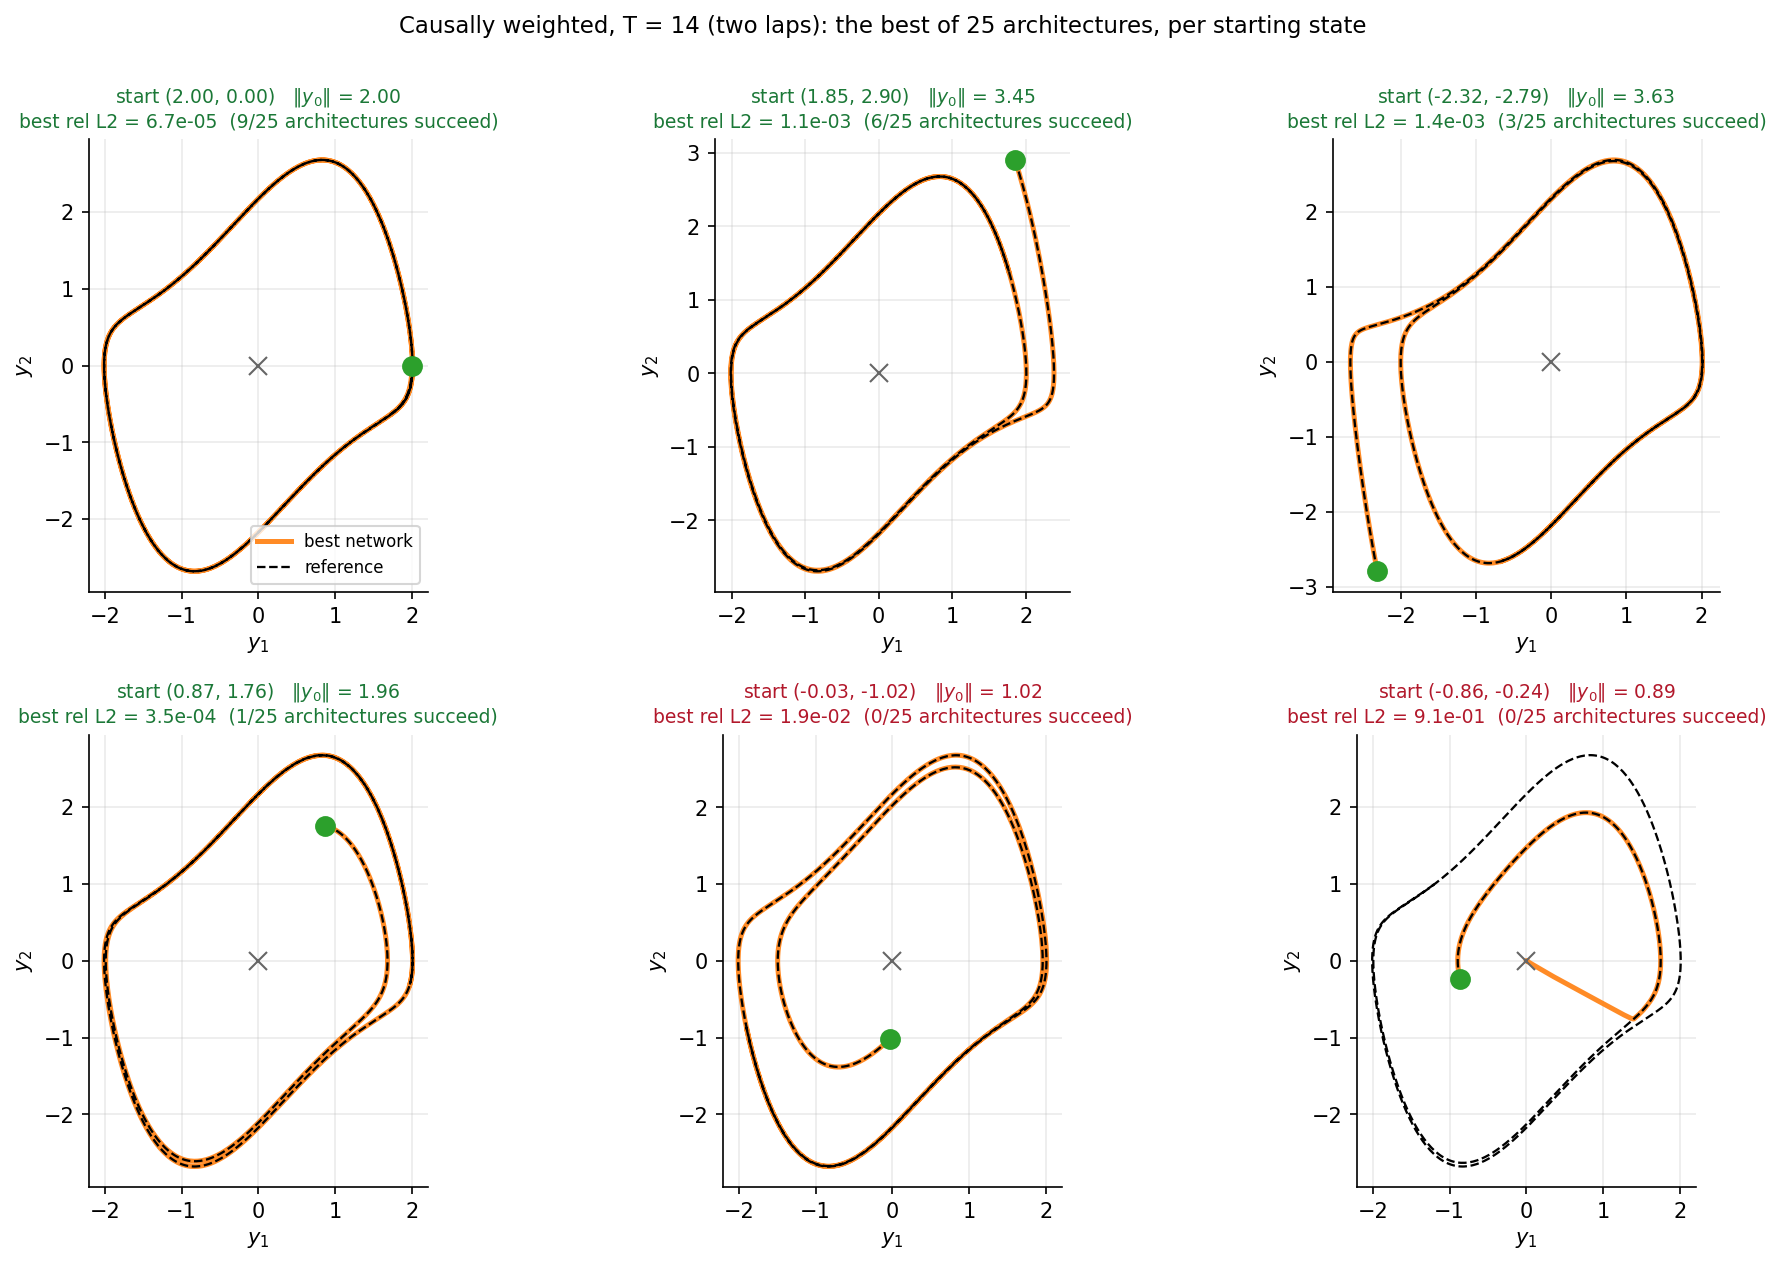
\includegraphics[width=\linewidth]{fig_start_gallery.png}
  \caption{Best causally weighted $T=14$ run (of 25 architectures) for
  each of the six starting states, in the phase plane: the outer starts
  track the loop; the inner starts, those nearest the repelling
  equilibrium, are never solved by any architecture.}
  \label{fig:start-gallery}
\end{figure}

\begin{figure}[tbp]
  \centering
  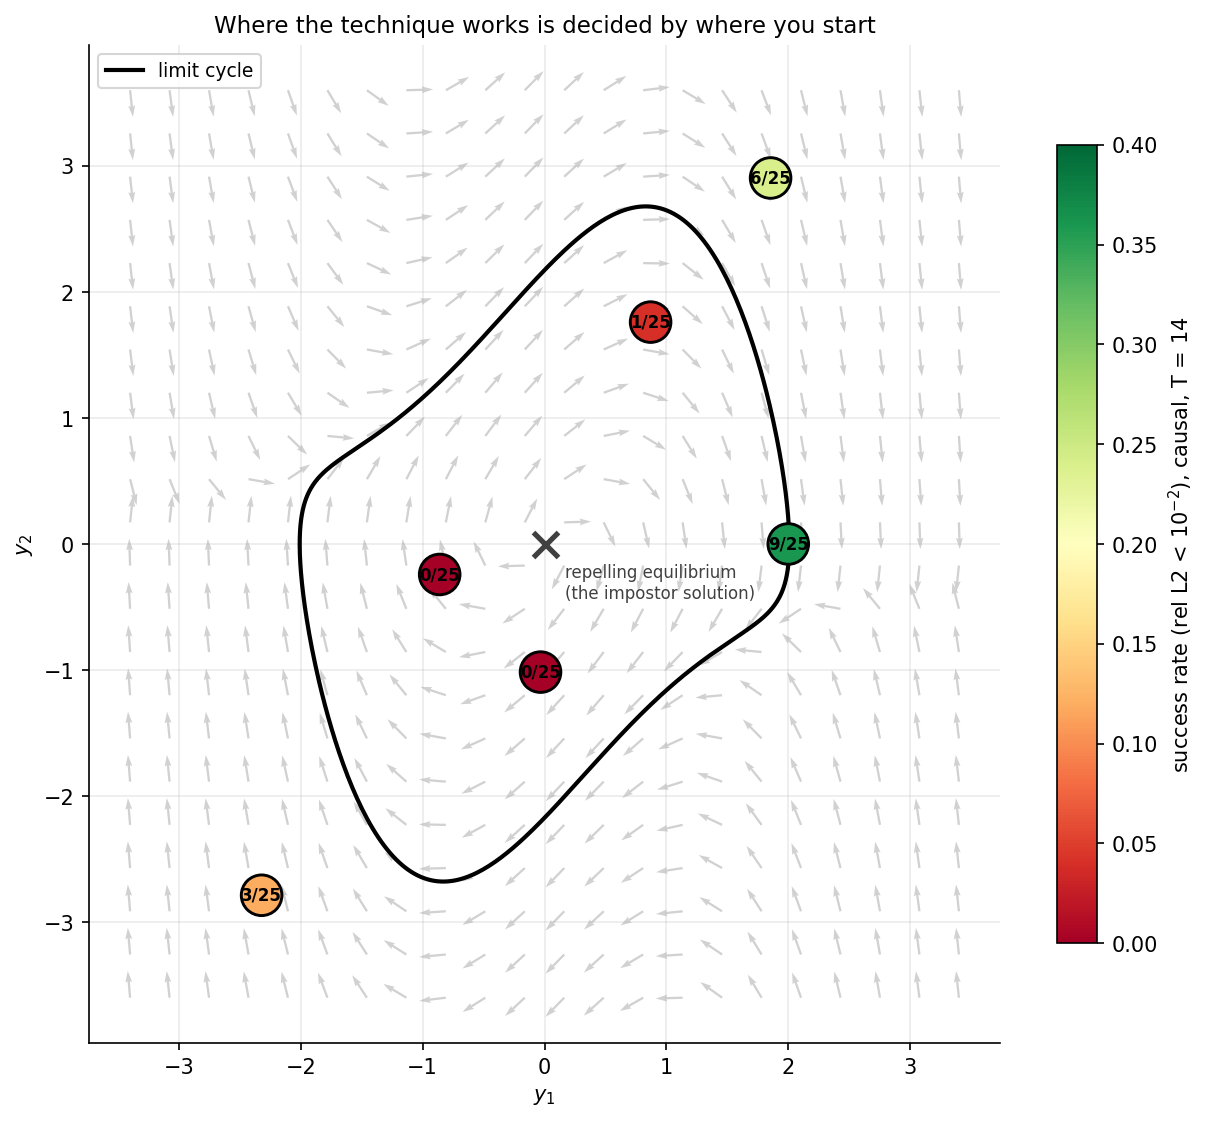
\includegraphics[width=0.72\linewidth]{fig_success_map.png}
  \caption{The six starting states drawn on the vector field, coloured by
  success rate: the geometry of the failure. Success falls off toward the
  repelling equilibrium.}
  \label{fig:success-map}
\end{figure}

\subsection{Collocation density}
\label{sec:density}

The remaining resource axes are the collocation points themselves: how
many, and where. I cross densities $\{5, 80, 320\}$
points per unit time (with density 20 imported from
Sections~\ref{sec:cont-results} and~\ref{sec:causal} rather than rerun)
with horizons $T \in \{7, 14, 27, 40\}$, three seeds and both arms: 72
new runs. I placed two hypotheses on record before the sweep:
\begin{itemize}
  \item[H1:] the plain arm is density-independent at the failing horizons,
  because the mean in Eq.~\eqref{eq:contloss} amortises the escape
  window's cost regardless of how many points share it;
  \item[H2:] the causal arm is density-sensitive, through the
  between-points loophole of Section~\ref{sec:causal}.
\end{itemize}

\begin{table}[tbp]
  \centering
  \caption{Relative $L_2$ error against collocation density (points per
  unit time); medians over three seeds. ``cw'' marks runs whose causal
  front certified arrival on a wrong solution (certified-wrong).}
  \label{tab:density}
  \small
  \begin{tabular}{clllll}
    \toprule
    arm & $T$ & $d = 5$ & $d = 20$ & $d = 80$ & $d = 320$ \\
    \midrule
    plain  & 14 & $0.913$ & $0.793$ & $0.790$ & $0.792$ \\
    plain  & 27 & $0.915$ & $0.904$ & $0.905$ & $0.904$ \\
    plain  & 40 & $0.943$ & $0.942$ & $0.942$ & $0.941$ \\
    \addlinespace
    causal & 7  & $0.754$ (cw 3/3) & $7.6\times10^{-5}$ & $7.9\times10^{-5}$ & $9.7\times10^{-5}$ \\
    causal & 14 & $0.974$ (cw 2/3) & $2.1\times10^{-4}$ (worst $0.71$) & $1.8\times10^{-4}$ & $1.9\times10^{-4}$ \\
    causal & 27 & $2.70$ & $1.90$ & $1.45$ & $1.45$ \\
    causal & 40 & $2.89$ & $2.04$ & $2.05$ & $2.05$ \\
    \bottomrule
  \end{tabular}
\end{table}

H1 is confirmed sharply (Table~\ref{tab:density} and
Figure~\ref{fig:density}): across a 64-fold density range the plain-arm
medians at the failing horizons move by factors of 1.15, 1.01 and
1.003. Collocation cost was never the binding limit, and this is now a
direct measurement rather than an affordability argument. H2 refines into
a threshold. Below roughly 20 points per unit time the causal certificate
is actively misleading: at density 5 the front ``arrives'' in about 12k
steps onto wrong solutions (certified-wrong in three of three seeds at
$T=7$), because the gaps are so wide the quarantine has nothing to hold
(Figure~\ref{fig:density-front}). At density 20 and above, the one-period
error collapses to $\sim\!10^{-4}$ and stays flat to 320, with a
density-independent crossing cost, exactly as the $\varepsilon$
normalisation of Eq.~\eqref{eq:causal} intends. Density does buy one real
thing at two periods: reliability. At density 20 one seed in three fails
($0.71$); at 80 and 320 all seeds land at ${\sim}2\times10^{-4}$, closing
the between-points loophole. At four and six periods density changes
nothing: the causal wall stays at 1.45--2.9 from 5 to 320 points per unit
time.

\begin{figure}[tbp]
  \centering
  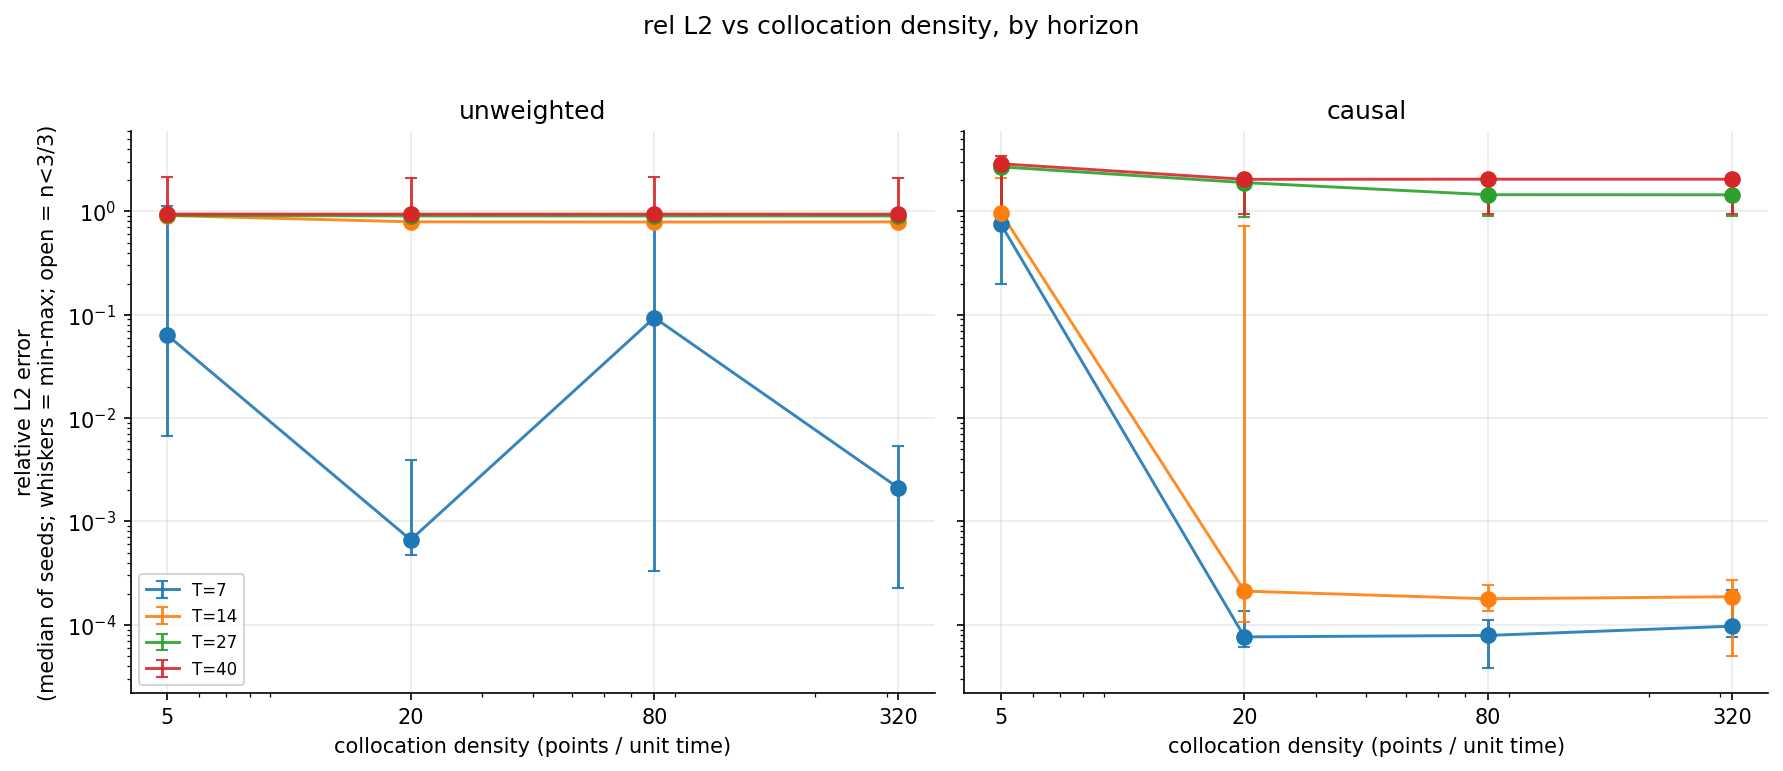
\includegraphics[width=\linewidth]{fig_density.png}
  \caption{Relative $L_2$ error against collocation density (logarithmic
  axis), one line per horizon, plain (left) and causal (right); medians
  with min--max whiskers. The plain lines are flat everywhere; the causal
  lines fall off a cliff between density 5 and 20 at the rescued horizons
  and stay flat beyond it, and they stay high at the failing horizons.}
  \label{fig:density}
\end{figure}

\begin{figure}[tbp]
  \centering
  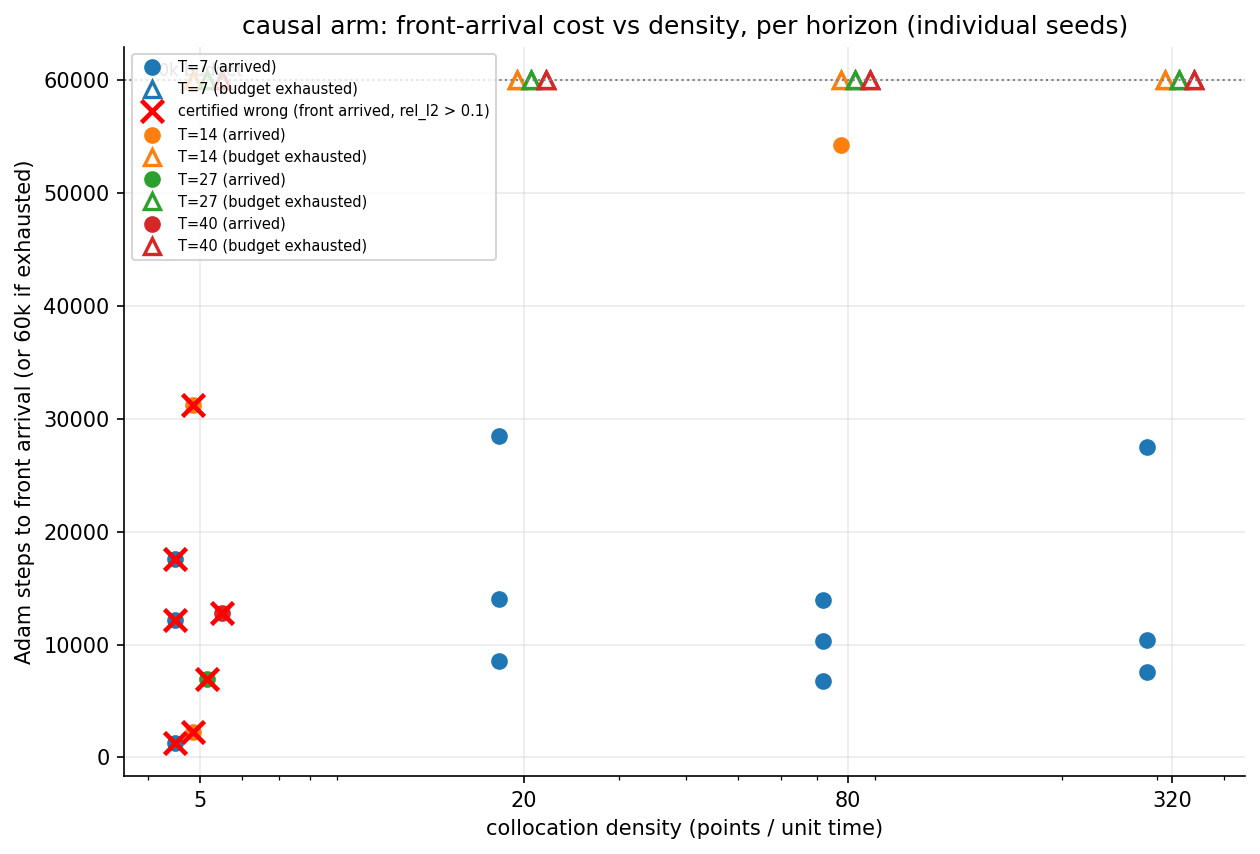
\includegraphics[width=0.8\linewidth]{fig_density_front.png}
  \caption{The causal front's arrival cost against density, with
  certified-wrong runs marked: at density 5 the front arrives cheaply on a
  wrong solution; at density 20 and above the arrival cost is
  density-independent. The crossing cost is set by the physics, not by
  the number of points.}
  \label{fig:density-front}
\end{figure}

\subsection{Collocation placement}
\label{sec:placement}

Both measured loopholes look like placement artefacts: the
starved-causal escape of Section~\ref{sec:causal} lives in the unsampled
interval immediately after the anchor, before the first collocation point,
and the plain arm's escape becomes visible 1.5--3 time units in. I hold
the density fixed at 20 and compare two alternative
placements against the Latin-hypercube baseline: \emph{uniform}
(deterministic bin midpoints) and \emph{anchored} (Latin hypercube plus 40
extra points packed geometrically into $(10^{-3}, 1]$, a direct plug of
the first-gap escape), each crossed with both arms, $T \in \{14, 27\}$ and
three seeds: 24 runs.

The plain arm is placement-independent at both horizons (medians
0.786--0.806 at $T=14$, 0.901--0.910 at $T=27$, indistinguishable from
the baseline). In the causal arm at $T=14$, uniform and anchored
placements both land three of three seeds at $\le 3\times10^{-4}$ where
the baseline went two of three, so placement was never the problem; the
baseline's bad seed was luck. And at $T=27$ anchoring does not rescue the
four-period wall: best anchored seed 0.900 (others 0.900 and 1.96);
uniform 0.901, 2.85, 1.99 (Figure~\ref{fig:placement}). Plugging the gap
the escapes were seen to use does not prevent the failure: the escape is a
symptom of a front that never crossed rather than the cause of the
failure. Together with Section~\ref{sec:density} this closes the
collocation axis: neither how many points nor where they sit moves the
long-horizon walls.

\begin{figure}[tbp]
  \centering
  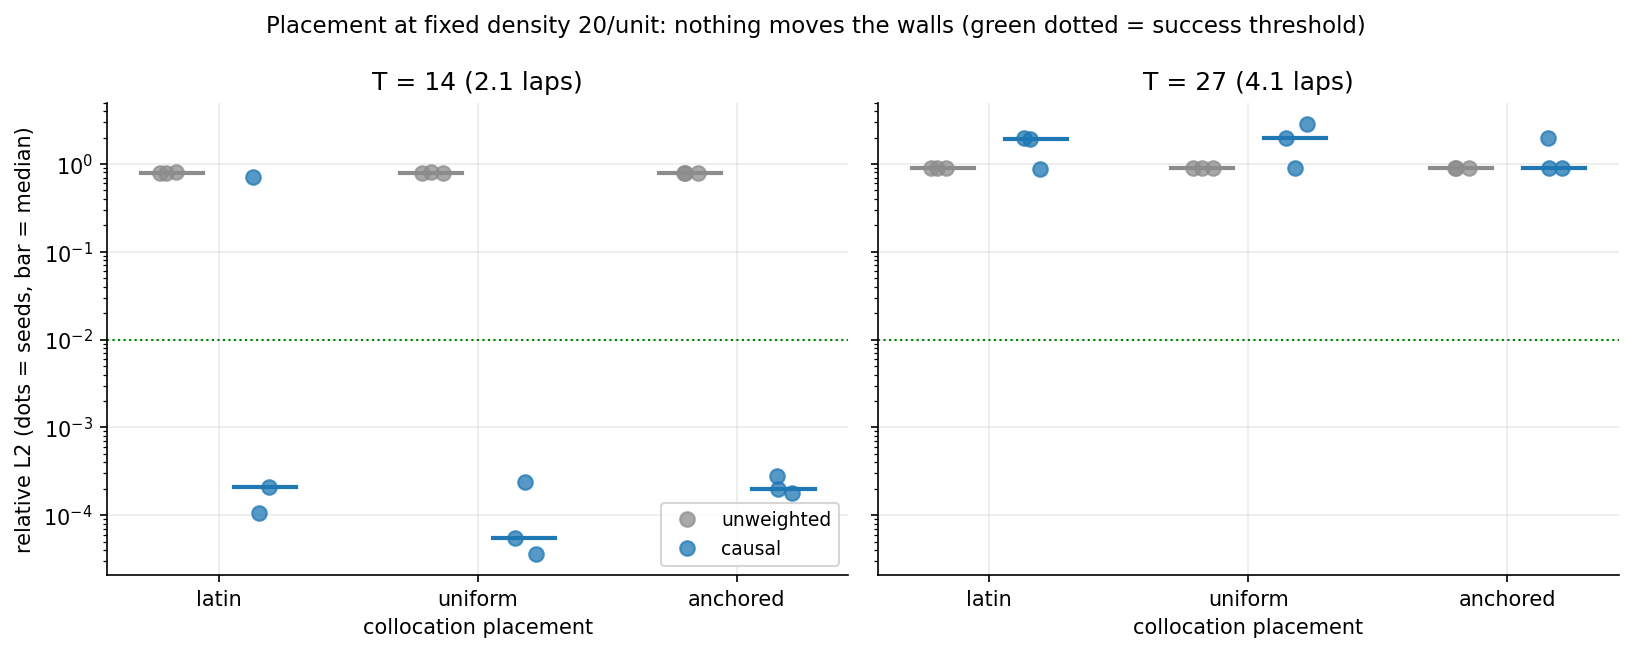
\includegraphics[width=\linewidth]{fig_placement.png}
  \caption{The placement comparison at both horizons and arms: three
  placements, indistinguishable walls.}
  \label{fig:placement}
\end{figure}

\subsection{What the continuous-time route establishes}
\label{sec:cont-summary}

The continuous-time formulation works, per starting state, up to a wall
that no resource moves. It reproduces the source work's accuracy below one
period; causal weighting, the strongest known loss-level fix, moves the
wall from one period to two and makes failures detectable; and beyond
that, optimisation budget ($4\times$, zero of seven), network size (600
runs, depth harmful), collocation density (64-fold range) and collocation
placement (targeted) are all null axes. The one variable that orders
outcomes is the starting state's position relative to the repelling
equilibrium: success at two periods is a 12.7\% geometry-dependent gamble
at the 1\% bar, and at four periods no run wins it. This is the complete,
measured case for imposing the physics structurally instead, which is the
discrete-time formulation of the next section.

% ===========================================================================
\section{The discrete-time formulation}
\label{sec:disc-method}

\subsection{Implicit Runge--Kutta background}

Integrating $\dot y = f(y)$ exactly across one step gives
\begin{equation}
  y(t + \Delta t) = y(t) + \int_t^{t+\Delta t} f\big(y(s)\big)\, ds ,
  \label{eq:step-integral}
\end{equation}
so a one-step numerical method is, at heart, a quadrature rule (a recipe
for approximating an integral from a few point evaluations) applied to
Eq.~\eqref{eq:step-integral}. The simplest choice, approximating the
integrand by its value at the left endpoint, is Euler's method,
$y^{n+1} = y^n + \Delta t\, f(y^n)$. Better quadrature needs the
integrand at interior times of the step; but the integrand is
$f(y(s))$, and $y(s)$ is exactly what is not yet known there. The
Runge--Kutta family resolves this circularity by introducing $q$
\emph{stage states}, internal estimates of the solution at chosen
fractions $c_1, \dots, c_q$ of the step, defined self-consistently
through each other:
\begin{equation}
  y^{n+c_j} = y^n + \Delta t \sum_{k=1}^{q} a_{jk}\, f\big(y^{n+c_k}\big),
  \qquad
  y^{n+1} = y^n + \Delta t \sum_{j=1}^{q} b_j\, f\big(y^{n+c_j}\big),
  \label{eq:irk}
\end{equation}
where the nodes $c$, matrix $A = (a_{jk})$ and weights $b$ form the Butcher
tableau, which is the method's complete identity card. If $A$ is strictly
lower triangular, each stage depends only on earlier ones and the step is
computed left to right: an explicit method (the sixth-order reference
integrator of Section~\ref{sec:problem} is one). When $A$ is full, every
stage depends on every other and the first relation of
Eq.~\eqref{eq:irk} is a genuine coupled system of $2q$ nonlinear
equations (two state components times $q$ stages): the method is
implicit, normally solved by a root-finder at every step.

Why pay the implicit price? Two properties, and both are load-bearing
here.
\begin{itemize}
  \item \textbf{Order.} A method has order $p$ if the error of one step
  shrinks like $\Delta t^{p+1}$, so that the accumulated error over a
  fixed interval shrinks like $\Delta t^{p}$; halving the step of an
  order-6 method cuts the error 64-fold. Gauss--Legendre tableaus place
  the nodes $c_j$ at the roots of the degree-$q$ Legendre polynomial
  mapped to $[0,1]$, the same points that make Gaussian quadrature exact
  for polynomials of degree $2q-1$, and attain order $2q$, the maximum
  any $q$-stage method can achieve: each added stage buys two orders.
  \item \textbf{A-stability.} Stability is probed on the linear test
  equation $\dot y = \lambda y$ with $\mathrm{Re}\,\lambda < 0$, whose
  true solution decays; a method is A-stable if its numerical solution
  also decays at every step size. Explicit methods never are (too large
  a step and the numerical solution explodes although the true one
  decays), while Gauss--Legendre methods are A-stable at every
  order~\cite{hairer1996}. A-stability is, however, a \emph{linear}
  property: on a nonlinear system the implicit stage equations must also
  have a findable solution, and that solvability, not stability, is
  what breaks first as the step grows (measured directly in
  Section~\ref{sec:disc-routes}).
\end{itemize}
Gauss--Legendre methods are also collocation
methods in the classical sense: there is a single
degree-$q$ polynomial through $y^n$ that satisfies the differential
equation exactly at the $q$ node times, and the stages are its values
there, so the stage states approximate the solution at the interior
times $c_j\,\Delta t$ to high order. They are not abstract
intermediates (Figure~\ref{fig:anatomy}).

\begin{figure}[tbp]
  \centering
  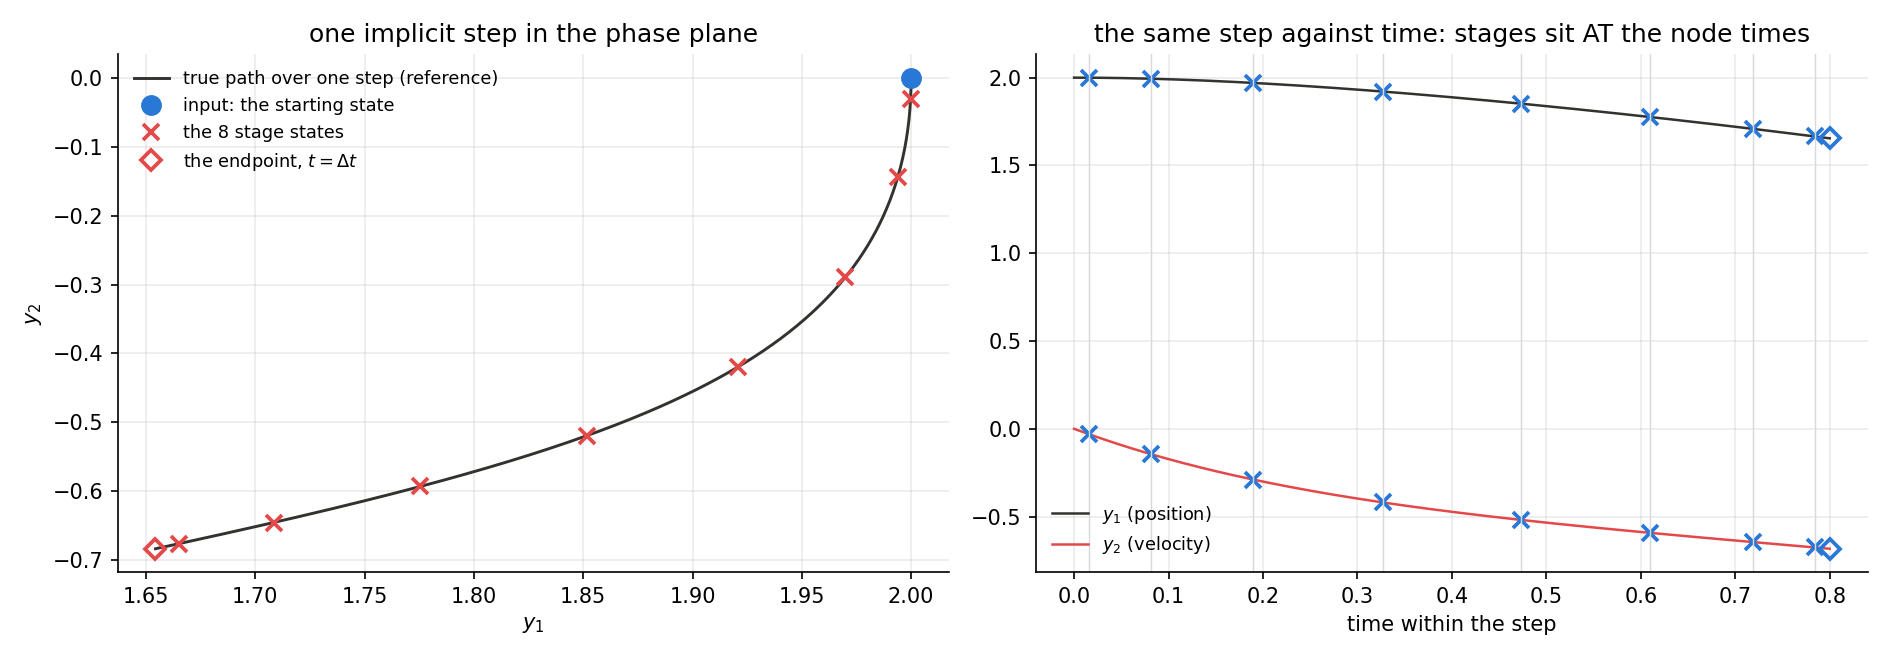
\includegraphics[width=0.8\linewidth]{fig_step_anatomy.png}
  \caption{Anatomy of one implicit step from $(2,0)$ at $q=8$: the true
  path over $[0, 0.8]$, the eight Gauss stage states (exact solver), and
  the endpoint. The stages lie on the true mini-trajectory, crowding toward
  the ends of the step where the Legendre roots sit. Given the input state,
  the network must place all nine points.}
  \label{fig:anatomy}
\end{figure}

\subsection{The loss}

The source work's discrete-time construction replaces the root-finding
solve of Eq.~\eqref{eq:irk} by a network that proposes all $q+1$ unknowns
at once; each defining relation is rearranged to isolate the known state,
\begin{equation}
  \underbrace{y^{n+c_j} - \Delta t \sum_k a_{jk} f\big(y^{n+c_k}\big)}_{\text{reconstruction } j} = y^n
  \qquad\text{and}\qquad
  \underbrace{y^{n+1} - \Delta t \sum_j b_j f\big(y^{n+c_j}\big)}_{\text{reconstruction } q+1} = y^n ,
  \label{eq:recon}
\end{equation}
so that if the network's outputs really are the stage states of the scheme,
all $q+1$ reconstructions land exactly on $y^n$. The loss I use is the
mean of the squared reconstruction mismatches over outputs, components and
batch.
(In the source work the loss is a sum rather than a mean and carries an
additional boundary term; for an ordinary differential equation there is no
boundary, and at fixed batch size the mean is a rescaled sum. Both
differences are noted for exactness.) Nothing else is supervised: there is
no time derivative of the network, no collocation grid over time, and no
trajectory data. The tableau is fixed and known; only the stage values are
learned. The anchoring that the continuous-time formulation concentrates
in a single point is here built into every term of the loss: every output
is tied to a known state through the algebra of the step.

\subsection{The state as the input: a reusable flow map}

In the source work the network input is a spatial coordinate and the known
$y^n$ is a measured snapshot of a field; an ordinary differential equation
has no spatial coordinate, so the input becomes \emph{the starting state
itself}: the network maps $(y_1, y_2)$ to the $q$ stage states plus the
endpoint, $2(q+1)$ numbers. Trained over a region of starting states, one
network becomes a reusable flow map for the fixed step: feed in any state
and receive the state $\Delta t = 0.8$ later; feed the endpoint back in
and a whole trajectory follows, without retraining. This differs from the
sequential mode described in the source work, which retrains at every step.
The generalisation itself follows Fern\'andez Corral et
al.~\cite{fernandez2024}, who apply it to conservative and periodically
forced systems; the dissipative limit-cycle instantiation, the
exact-scheme error attribution, the seed and selection analysis, and the
head-to-head comparison with the continuous-time formulation below are, to
my knowledge, new.

\subsection{Protocol and guardrails}
\label{sec:guardrails}

I train on 2000 starting states per run, Latin-hypercube sampled over
the rectangle $y_1 \in [-2.5, 2.5]$, $y_2 \in [-3, 3]$, the limit cycle
with margin; a sampling region, not a boundary. (This is the discrete-time
analogue of the collocation budget of Section~\ref{sec:collocation}: the
equations are enforced at 2000 points of the \emph{state space}, rather
than on a grid in time.) The network body is identical to the
continuous-time experiments (4 hidden layers of 50 hyperbolic-tangent
units, double precision) with a linear output layer of $2(q+1)$ units;
only the output layer grows with $q$. At the headline $q = 8$ this means
18 outputs and $8{,}718$ trainable parameters, and the interior node
times of the step are
$c_j\,\Delta t = \{0.016, 0.081, 0.190, 0.327, 0.473, 0.610, 0.719,
0.784\}$, the Gauss--Legendre nodes of
Section~\ref{sec:disc-method} scaled by $\Delta t = 0.8$. Each input
component is scaled by its half-range ($y_1$ by 2.5 and $y_2$ by
3), the discrete-time analogue of the declared time rescaling of
Section~\ref{sec:cont-method}. The optimiser, restart discipline and
budget are identical to Section~\ref{sec:cont-protocol}, so differences
between the formulations are the formulation's. The sweep is
$q \in \{2, 4, 8, 16, 32\}$ times three seeds, fifteen runs.

Because the trained map will be judged against the scheme it imitates, the
scheme itself is verified first, independently of any network, in three
steps:
\begin{enumerate}
  \item the tableau is constructed for each $q$ from the Legendre roots
  and checked against every identity it must satisfy (row sums, quadrature
  exactness to degree $2q-1$, the collocation conditions, and a
  symplecticity identity that the construction does not impose); the
  worst violation up to $q = 32$ is $2\times10^{-16}$, machine precision;
  \item an exact solver (a root-finder on the $2q$ stage equations,
  convergence judged on the residual itself) then provides the scheme
  with no network in it, and its measured convergence order on problems
  with known solutions matches or exceeds the theoretical $2q$; and
  \item a single step of $0.8$ from 100 sampled states converged in 100
  of 100 cases at every $q$, establishing that the step is well-posed on
  the whole training region.
\end{enumerate}
Evaluation is on a held-out $21\times21$ uniform grid over
the rectangle (441 states, disjoint from the training samples by
construction, with the origin at its centre) and, for chained evaluation,
on a held-out test set of 108 starting states; all ground truths are
regenerated by the reference integrator, stopping exactly at each stage
time.

\subsection{Results: the error floor}
\label{sec:disc-results}

\begin{table}[tbp]
  \centering
  \caption{Endpoint relative $L_2$ error on the 441 held-out states versus
  the number of stages $q$ (median over three seeds), against the exactly
  solved scheme on the same states and metric.}
  \label{tab:floor}
  \small
  \begin{tabular}{ccc}
    \toprule
    $q$ (order $2q$) & trained network (median) & exact scheme, same grid \\
    \midrule
    2 (4)   & $3.94\times10^{-2}$ & $4.20\times10^{-2}$ \\
    4 (8)   & $4.57\times10^{-3}$ & $2.20\times10^{-4}$ \\
    8 (16)  & $3.61\times10^{-3}$ & $2.38\times10^{-8}$ \\
    16 (32) & $3.63\times10^{-3}$ & $8.9\times10^{-14}$ \\
    32 (64) & $3.63\times10^{-3}$ & $1.4\times10^{-13}$ \\
    \bottomrule
  \end{tabular}
\end{table}

\begin{figure}[tbp]
  \centering
  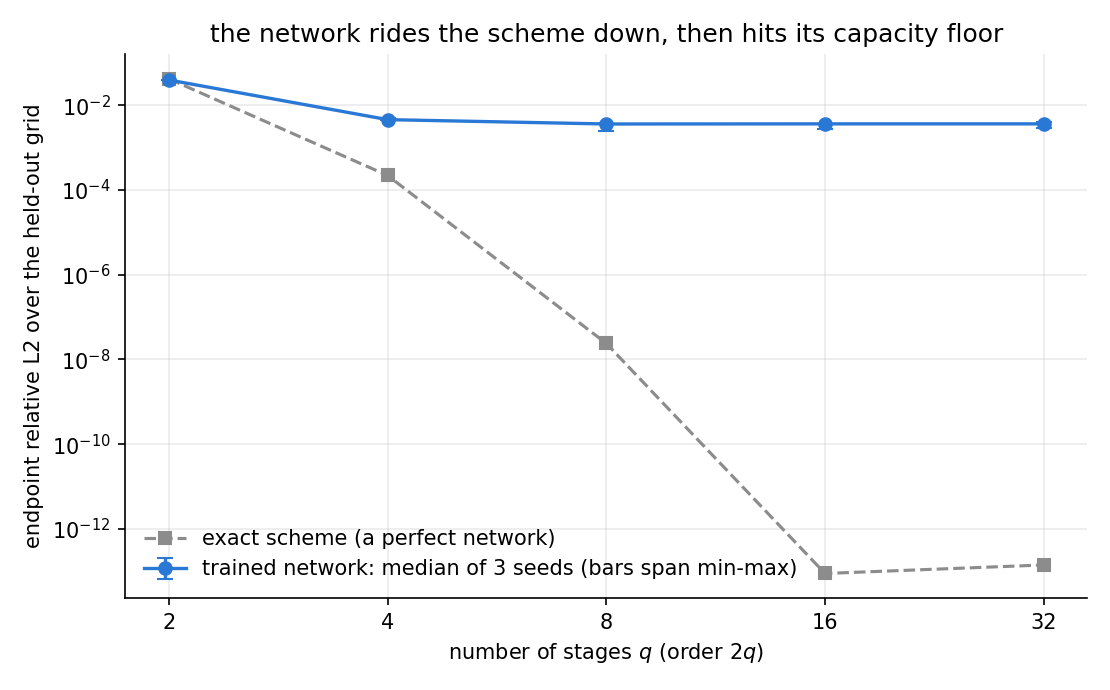
\includegraphics[width=0.72\linewidth]{fig_capacity_floor.png}
  \caption{Endpoint relative $L_2$ error versus number of stages: the
  trained network (median of three seeds, min--max whiskers) rides the
  scheme's error down and then flattens onto its floor, while the exactly
  solved scheme (grey) continues to machine precision.}
  \label{fig:floor}
\end{figure}

Training gives no trouble: all fifteen runs converge to
losses of $7\times10^{-6}$ to $2.6\times10^{-5}$ with no collapse and no
divergence, and, unlike every failed run of
Sections~\ref{sec:cont-results} and~\ref{sec:causal}, the loss is an
honest proxy for the error: a squared-residual loss of $10^{-5}$ resolves
outputs to roughly its square root, $3$--$5\times10^{-3}$, which is where
the held-out error lands.

Table~\ref{tab:floor} and Figure~\ref{fig:floor} give the central result
of this section. At $q = 2$ the trained network sits
\emph{on} the exactly solved scheme's own error: the map is
scheme-limited, and even a perfect fit would be that wrong. From $q = 4$
the curves part: the scheme plunges ten orders of magnitude to roundoff
while the network stays flat at $3.6$--$4.6\times10^{-3}$ (flat to a factor
$1.27$ for all $q \ge 4$, all seeds agreeing). The remaining error belongs
to the network rather than the scheme, so more stages cannot help; the
lever is the network itself, and Section~\ref{sec:disc-size} shows that
the binding constraint there is the optimisation rather than capacity. The
stages are learned as accurately as the endpoint at every $q$ (asking for
66 outputs at $q = 32$ instead of 18 at $q = 8$ degrades nothing), the
error is largest at the corners of the training region where the dynamics
are fastest, and the error maps of all three seeds share the same
structure. The floor is a property of the method rather than an
initialisation accident.

\subsection{The capped metric, and the error as a distribution}
\label{sec:disc-rho}

\begin{table}[tbp]
  \centering
  \caption{The capped metric of Eq.~\eqref{eq:rho} on the 441-state grid
  (median over three seeds of the per-run values; exactly one metric-capped
  point per run, the origin). The mean column is pinned at the origin's
  fixed $1/441$ cap contribution from $q \ge 4$ and resolves nothing below
  it; this is the reporting rule of Section~\ref{sec:metrics} in action.}
  \label{tab:rho}
  \small
  \begin{tabular}{ccc}
    \toprule
    $q$ & median $\rho$ & mean $\rho$ (origin-dominated) \\
    \midrule
    2  & $7.2\times10^{-5}$ & $3.5\times10^{-3}$ \\
    4  & $1.0\times10^{-5}$ & $2.3\times10^{-3}$ \\
    8  & $6.5\times10^{-6}$ & $2.3\times10^{-3}$ \\
    16 & $6.0\times10^{-6}$ & $2.3\times10^{-3}$ \\
    32 & $5.1\times10^{-6}$ & $2.3\times10^{-3}$ \\
    \bottomrule
  \end{tabular}
\end{table}

In the capped metric (Table~\ref{tab:rho}) the median column tracks the
floor: $\sqrt{6.5\times10^{-6}} \approx 2.5\times10^{-3}$ at the headline
$q=8$, consistent with the relative $L_2$ floor as it must be. On the test
set (108 held-out starting states, each chained 50 steps, six periods, by
the three headline networks, 16{,}200 (state, time, seed) values) not a
single value reaches the cap: the pooled median is $1.8\times10^{-4}$ at
two periods and $1.7\times10^{-3}$ at six, the worst single value anywhere
in the set is $6.6\times10^{-2}$, and the smallest true state modulus
encountered is $0.063$, so the metric is defined everywhere with no
exclusions (Figure~\ref{fig:testset}).

\begin{figure}[tbp]
  \centering
  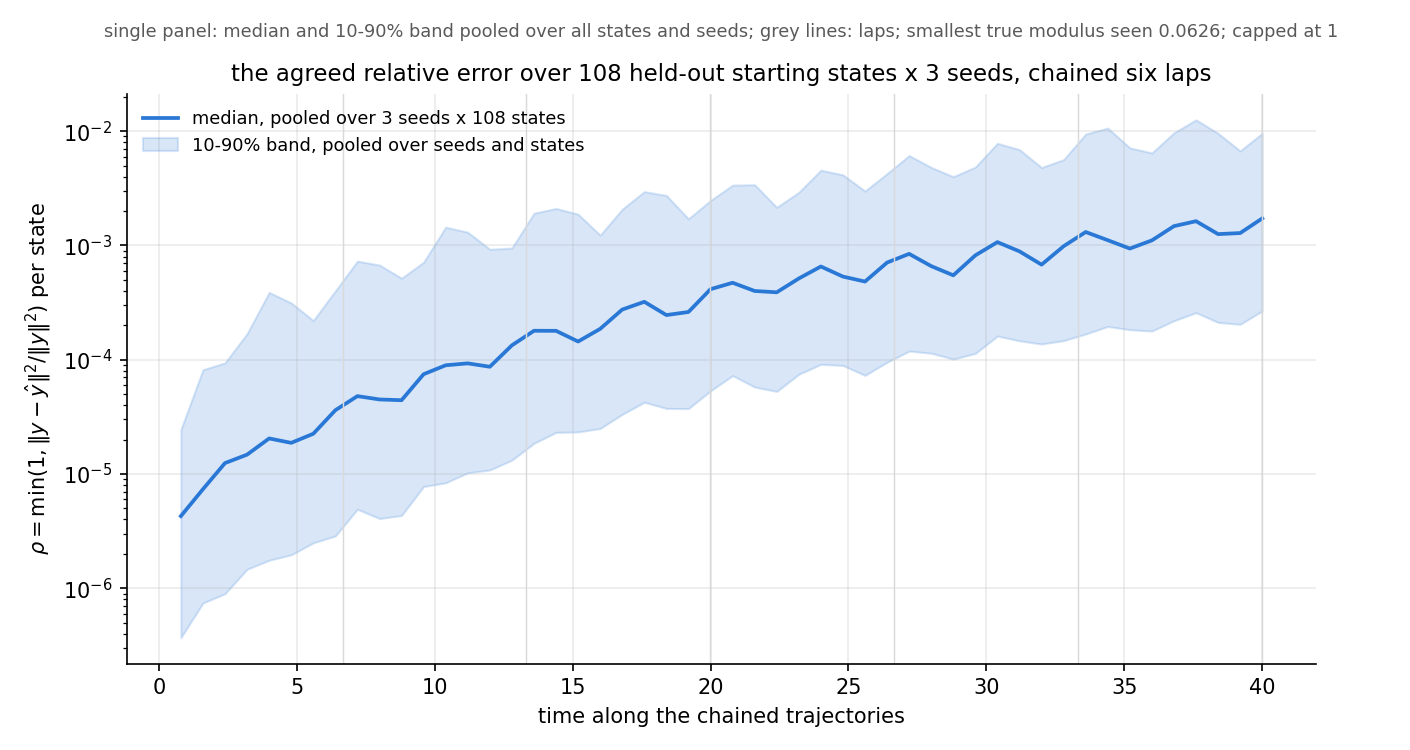
\includegraphics[width=\linewidth]{fig_test_set.png}
  \caption{The error as a distribution rather than a single trajectory:
  the capped metric $\rho$ over the pooled test set (three seeds
  $\times$ 108 held-out starting states, each chained 50 steps) against
  time; median and 10--90\% band. Tight, bounded, period-periodic drift;
  nothing excluded.}
  \label{fig:testset}
\end{figure}

\subsection{Network size, the seed, and selection}
\label{sec:disc-size}

The continuous-time route's size study has a discrete-time twin, with a
different verdict to test: is the $3.6\times10^{-3}$ floor a capacity
limit? The design crosses depth $\{2,\dots,10\}$ with width
$\{16, 32, 64, 128, 256\}$ (45 architectures) at fixed $q = 8$, three
seeds each, 135 runs, everything else frozen; each network is scored
one-step on the 441-state grid and chained fifty steps (six periods) over
the 108-start test set. A ten-seed replication over seven selected
architectures followed (70 runs, of which 52 fresh). For honesty the data
are split three ways: the 2000 training states; a separate set of
validation starts used only to choose among trained networks; and the
held-out test set, which no decision ever touches, so the reported
numbers cannot be flattered by the selection. Four findings.

\emph{The floor does not move.} The best of 45 architectures
(3 layers $\times$ 128 units) reaches $2.5\times10^{-3}$, a factor 1.5
below the 4$\times$50 baseline's $3.6\times10^{-3}$, and still five orders
of magnitude above the exact scheme (Figure~\ref{fig:size-map-discrete}).
Depth beyond about 5 hurts sharply (depths 2--5: median $4.6\times10^{-3}$;
depths 7--10: median $1.8\times10^{-2}$); width saturates at 64--128; the
worst corner (10 $\times$ 16) sits at $1.3\times10^{-1}$.

\emph{The binding constraint is the optimiser, not capacity.} Across the
135-run grid, the Spearman rank correlation between converged training
loss and held-out error (the correlation of the two quantities' rank
orderings, so that $+1$ means the run with the $k$-th smallest loss also
has the $k$-th smallest error for every $k$) is $+0.974$: architectures
that fail also fail to train. There is no capacity-rich,
badly-generalising regime, and every run used its full restart budget. The
floor of Section~\ref{sec:disc-results} is an optimisation floor.

\emph{Long horizons are decided by the seed, not the architecture.} Error
growth under chaining (six-period $\rho$ over one-period $\rho$) varies
${\sim}13\times$ between seeds of a single architecture and
${\sim}300\times$ across the grid; the baseline architecture's ten-seed
median growth is $\times 28$, with only one seed in ten saturating. In the
ten-seed replication no architecture reliably saturates: only
2 $\times$ 64 and 4 $\times$ 64 survive multiple-comparison correction
against the baseline, and even their seed spreads span decades
(Figure~\ref{fig:seed-replication}).

\emph{But growth is a measurable, transferable property of the trained
network.} A validation chain to the target horizon predicts held-out
six-period error at Spearman $+0.98$ (against $+0.35$ for the training
loss or the one-step error, and $+0.67$ for a one-period chain). Hence the
selection protocol:
\begin{enumerate}
  \item train about ten seeds of the chosen architecture;
  \item chain each on about fifty validation starts to the target
  horizon; and
  \item keep the seed with the smallest validation error.
\end{enumerate}
Selection beats the median seed by 3--96$\times$ per architecture. The
selected network, 4 layers $\times$ 32 units, seed 9, reaches six-period
$\rho = 2.0\times10^{-6}$ on the 108-start test set; on 20 fresh starts it
holds $\rho = 3.1\times10^{-6}$ at six periods and $3.4\times10^{-6}$ at
thirty periods ($t = 200$; growth $1.1\times$)
(Figure~\ref{fig:selection}). One measured caveat: a six-period validation
window does not certify thirty periods for every candidate (one
architecture's six-period winner creeps by a factor 8.7 by period 30); the
protocol's window should match the target horizon.

\begin{figure}[tbp]
  \centering
  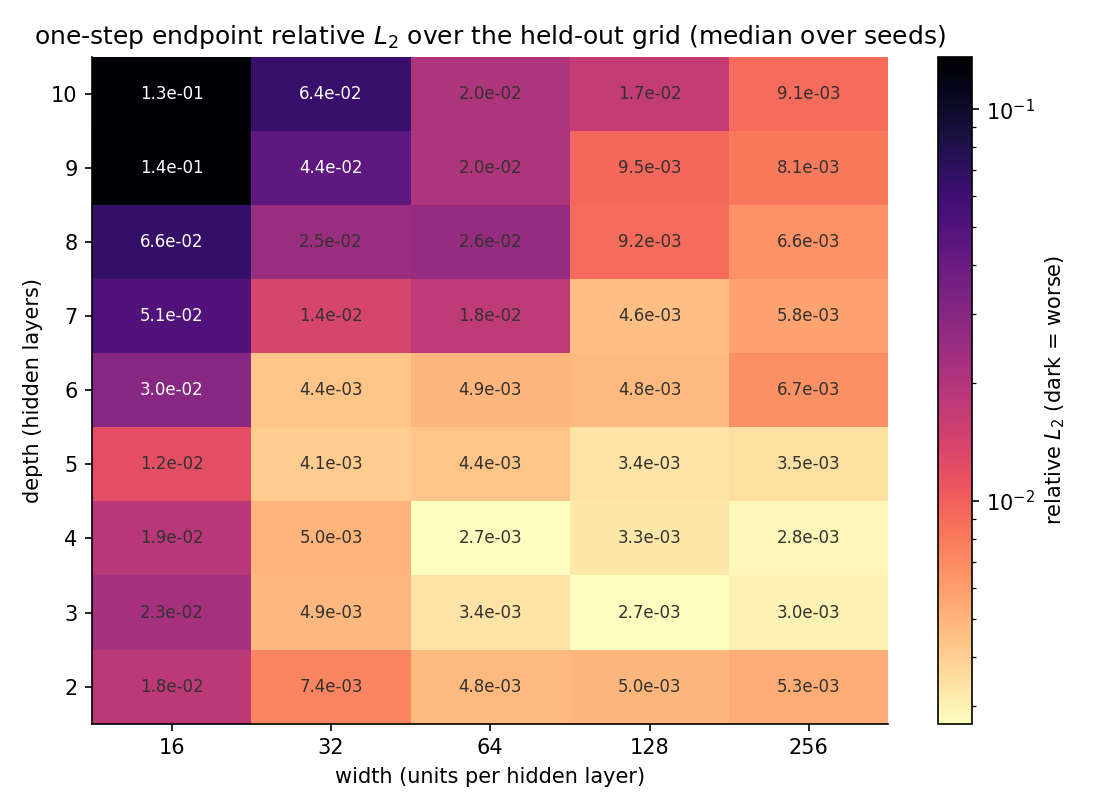
\includegraphics[width=\linewidth]{fig_size_map_discrete.png}
  \caption{One-step error over the architecture grid at fixed $q=8$: no
  cell approaches the exactly solved scheme; depth harms, width
  saturates. The floor is not a capacity floor.}
  \label{fig:size-map-discrete}
\end{figure}

\begin{figure}[tbp]
  \centering
  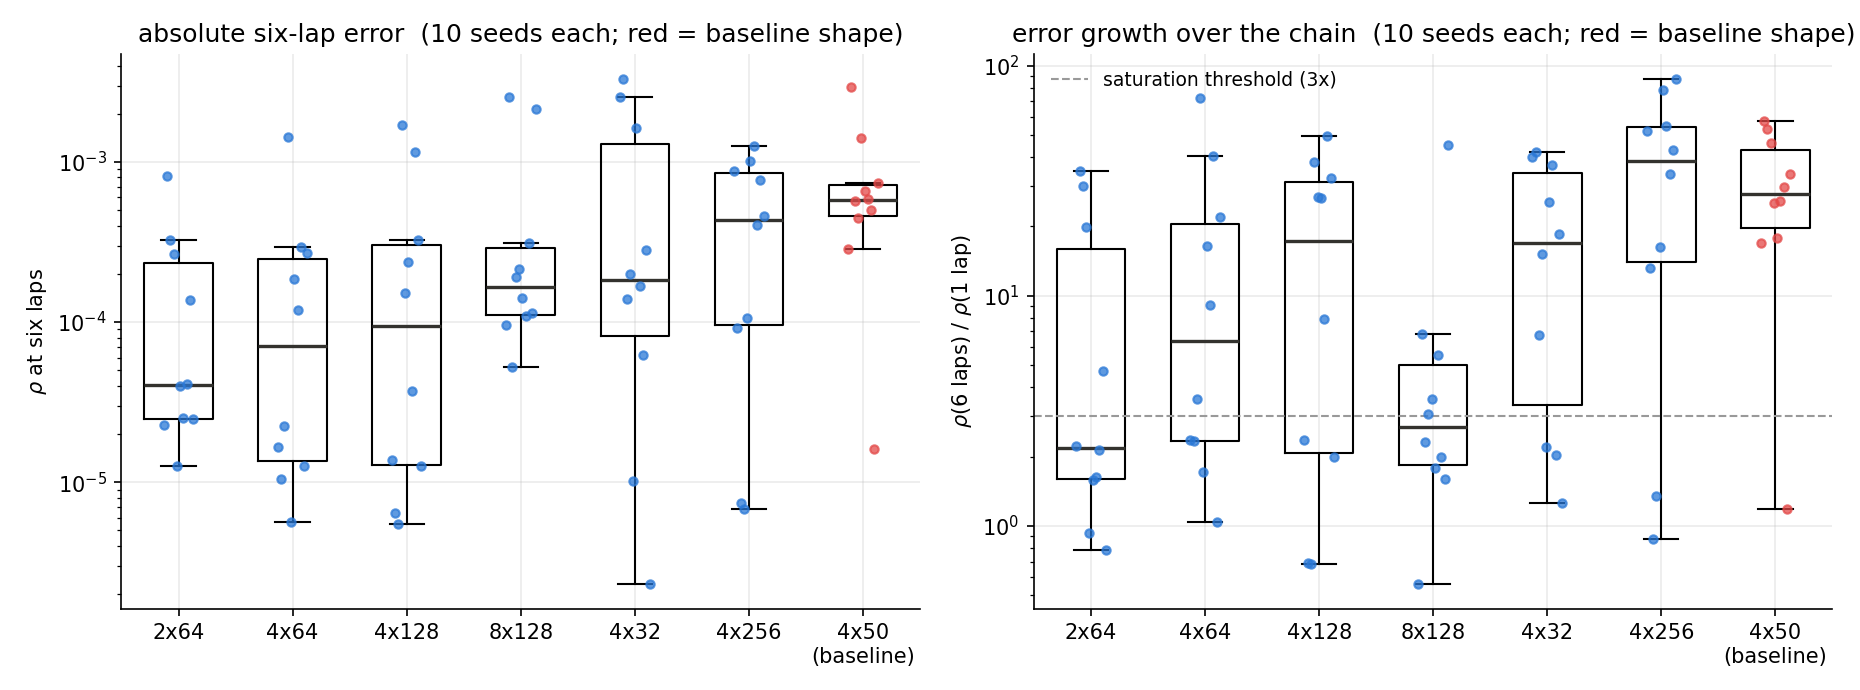
\includegraphics[width=\linewidth]{fig_seed_replication.png}
  \caption{Ten seeds for seven architectures, six-period chained error:
  the within-architecture seed spread rivals the whole grid's spread. The
  seed, not the shape, decides the horizon.}
  \label{fig:seed-replication}
\end{figure}

\begin{figure}[tbp]
  \centering
  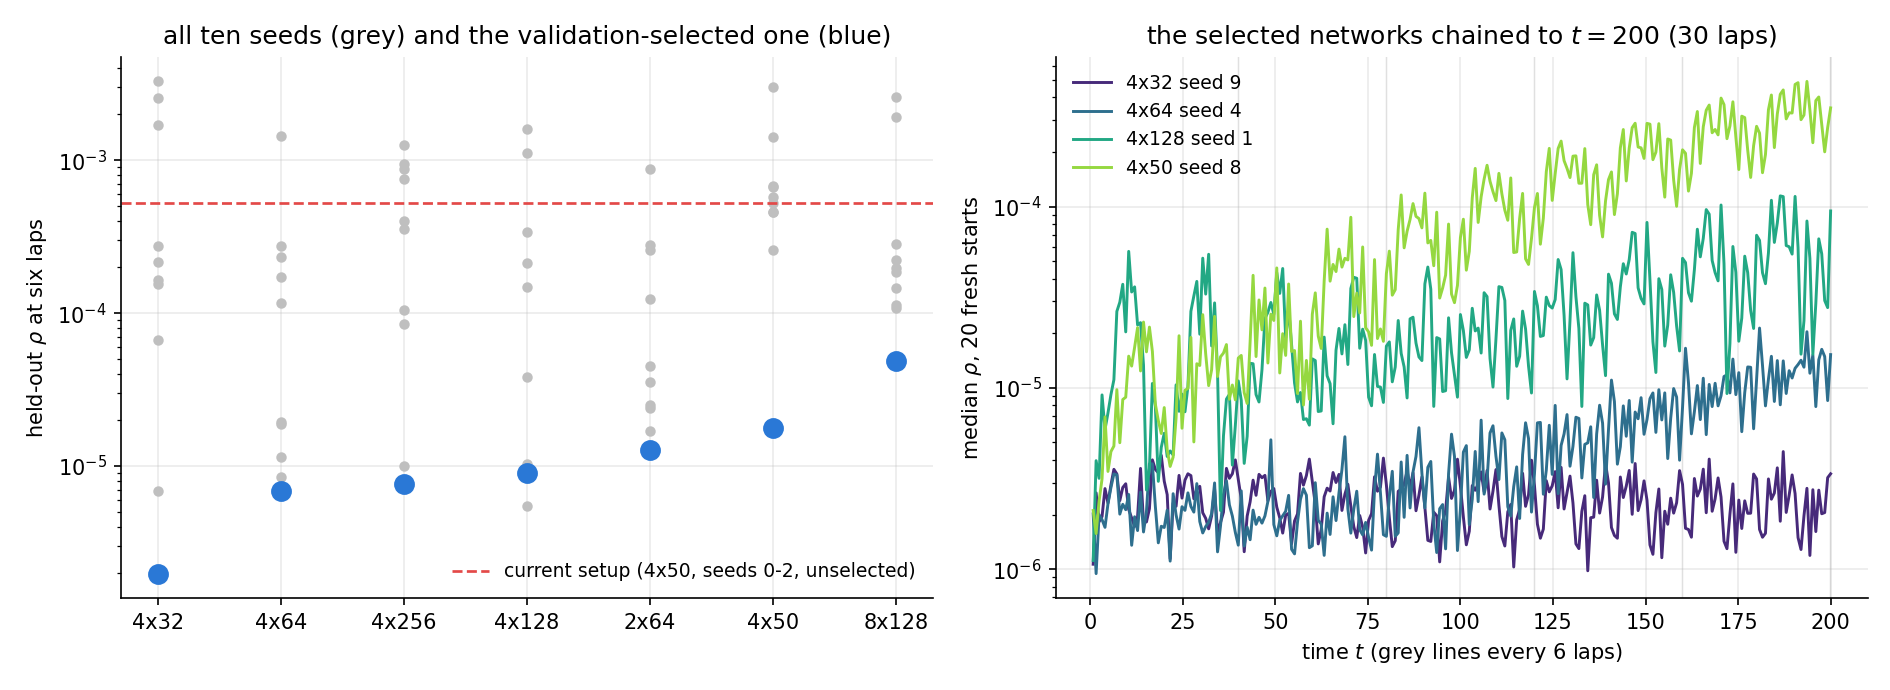
\includegraphics[width=\linewidth]{fig_selection.png}
  \caption{The selection payoff and the far-horizon check:
  validation-selected networks against their unselected siblings, and the
  selected 4 $\times$ 32 network holding $\rho \approx 3\times10^{-6}$
  flat to thirty periods on fresh starts.}
  \label{fig:selection}
\end{figure}

\subsection{Whole trajectories: chaining versus one giant step}
\label{sec:disc-routes}

How should the one-step technique deliver the actual goal, a starting
state in and a whole trajectory out? The source work's discrete-time
formulation can be read in two ways. Route A chains the trained one-step
map: feed the endpoint back in, no retraining, reaching a horizon $T$ in
$T / \Delta t$ applications of the network (50 chained steps of
$\Delta t = 0.8$ at $T = 40$, six periods). Route B generalises the
source work's Allen--Cahn mode: one network learns one \emph{giant}
implicit step whose stage states are the trajectory readout. Route B's
feasibility was checked first with the exact solver: at a full period
in one step ($\Delta t = 6.66$) the stage equations stop being reliably
solvable even at $q = 64$ (solver success 90 of 100 states). A-stability
is a linear property; what actually binds is nonlinear solvability.
The largest feasible giant step is half a period ($\Delta t = 3.2$ at
$q = 64$), and Route B was trained there (three seeds).

\begin{table}[tbp]
  \centering
  \caption{Whole trajectories over the continuous-time sweep's horizons:
  median relative $L_2$ error over the 108-start test set. The Route A
  columns chain the $\Delta t = 0.8$ map without retraining; the
  continuous-time column repeats the dedicated per-start fits of
  Sections~\ref{sec:cont-results} and~\ref{sec:causal} for scale.}
  \label{tab:routes}
  \small
  \begin{tabular}{cccl}
    \toprule
    $T$ & Route A, baseline (4$\times$50) & Route A, selected (4$\times$32) & continuous-time \\
    \midrule
    3  & $2.6\times10^{-3}$ & $1.6\times10^{-3}$ & $3.8\times10^{-5}$ (dedicated fit, one start) \\
    7  & $4.8\times10^{-3}$ & $2.1\times10^{-3}$ & $6.6\times10^{-4}$ (same caveat) \\
    14 & $9.0\times10^{-3}$ & $2.1\times10^{-3}$ & $0.79$ \\
    27 & $1.8\times10^{-2}$ & $2.1\times10^{-3}$ & $0.90$ \\
    40 & $2.6\times10^{-2}$ & $2.0\times10^{-3}$ & $0.94$ \\
    \bottomrule
  \end{tabular}
\end{table}

Table~\ref{tab:routes} and Figures~\ref{fig:headtohead}
and~\ref{fig:route-a-selected} give the result. The baseline seeds
compound gently, from $2.6\times10^{-3}$ at half a period to
$2.6\times10^{-2}$ at six; the selected network's column is flat at
$1.6$--$2.1\times10^{-3}$ from half a period to six periods (endpoint over
start: growth $1.3\times$). The map has stopped compounding, and at six
periods it is twelve times better than the best unselected seed. Against
Route B at the matched horizon ($T = 3.2$, i.e.\ four chained steps of
$0.8$ against one giant step of $3.2$): Route A selected
$2.1\times10^{-3}$ versus Route B $2.0\times10^{-2}$, so chaining beats
the one-shot mode by a factor 10 (already 6.6$\times$ with the unselected
seeds, $3.0\times10^{-3}$ versus $2.0\times10^{-2}$;
Figure~\ref{fig:route-b-vs-a}). Chained trajectories may briefly leave the
training rectangle (4 starts of 108, per seed); all return within one
step. The loop's attraction self-corrects the radial direction, and the
surviving error is mostly slow drift in oscillation phase, visible as the
settled period: $6.6573$ measured against the true $6.663287$
($-0.09\%$).

Two caveats apply to the comparison with the continuous-time column.
The continuous-time error is evaluated on the dense reference grid while
the chained error is evaluated at the step times, and each
continuous-time network was trained for its specific horizon and single
starting state while a single discrete map serves all horizons and all
108 starts: the comparison is between formulations rather than matched
estimators. The flip side is also visible in
Table~\ref{tab:routes}: below one period the dedicated continuous-time
fit is up to forty times more accurate, a dedicated single-trajectory
fit against a domain-wide generalist, with the crossover just past one
period.

\begin{figure}[tbp]
  \centering
  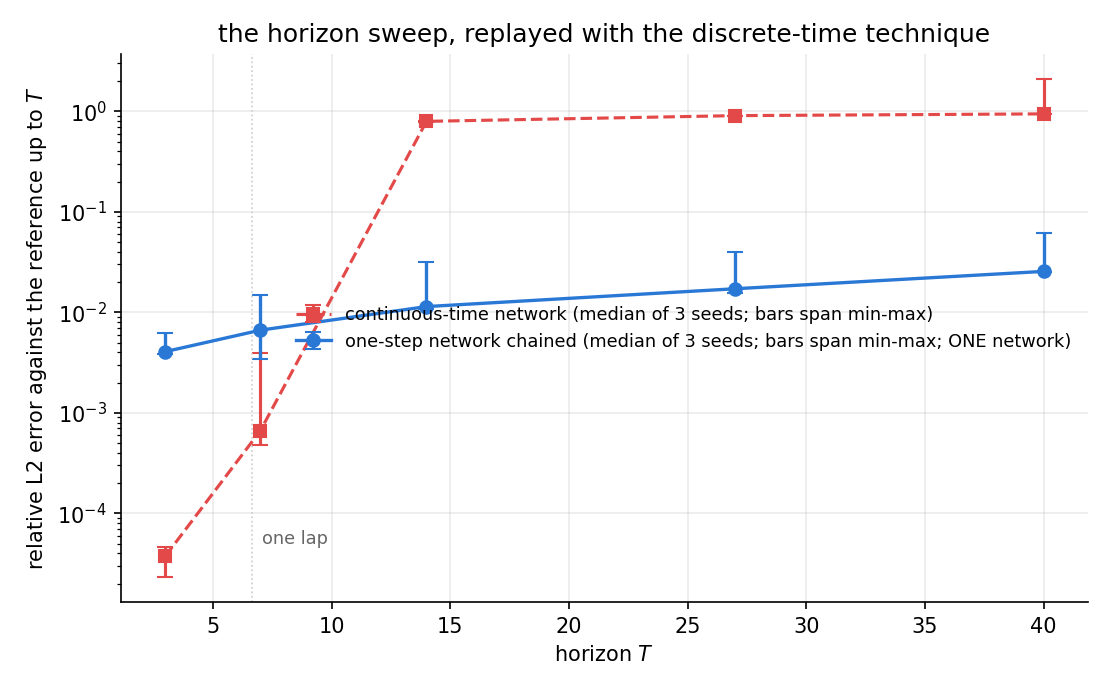
\includegraphics[width=0.8\linewidth]{fig_head_to_head.png}
  \caption{Both formulations on one axis, at the continuous-time sweep's
  exact horizons: the chained map rises gently where the continuous-time
  formulation fails at order one; below one period the dedicated
  continuous-time fit is the more accurate, with the crossover just past
  one period.}
  \label{fig:headtohead}
\end{figure}

\begin{figure}[tbp]
  \centering
  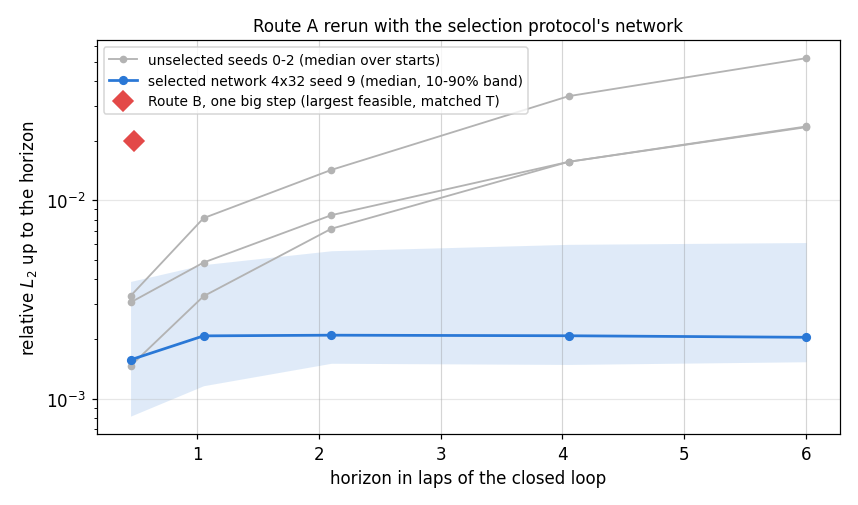
\includegraphics[width=\linewidth]{fig_route_a_selected.png}
  \caption{The selected network against the unselected baseline seeds,
  chained over the test set: a compounding
  $2.3$--$5.2\times10^{-2}$ six-period map becomes a flat
  $2.0\times10^{-3}$ one.}
  \label{fig:route-a-selected}
\end{figure}

\begin{figure}[tbp]
  \centering
  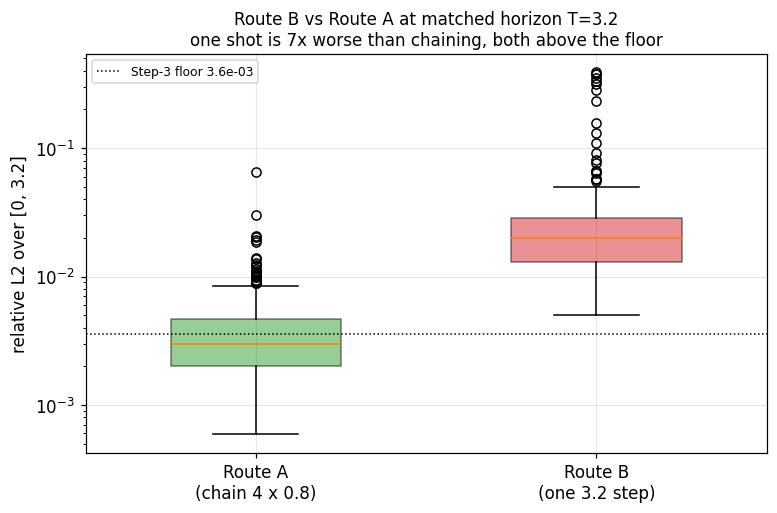
\includegraphics[width=\linewidth]{fig_route_b_vs_a.png}
  \caption{Route B (one giant half-period step, stage states as the
  trajectory readout) against Route A at the matched horizon: the one-shot
  mode is an order of magnitude worse, and a full-period step is not even
  reliably solvable.}
  \label{fig:route-b-vs-a}
\end{figure}

\subsection{What the physics buys: a data-supervised baseline}
\label{sec:baseline}

If perfect solution data were available, would it beat the physics? The
test is a matched pair: identical network, identical seeded initial
weights, identical optimiser and budget; the only differences are the
loss, \emph{physics} (the reconstructions of Eq.~\eqref{eq:recon}, as
everywhere above) versus \emph{data} (mean squared error to the true
stage states and endpoint, computed by the reference integrator), and
the training-set size $n \in \{50, 125, 250, 500, 1000, 2000\}$, three
seeds each, 36 runs.

\begin{table}[tbp]
  \centering
  \caption{Physics-trained versus data-trained (perfect labels) at matched
  everything else: endpoint relative $L_2$ on the 441-state grid, medians
  over three seeds, against training-set size $n$. The last column is the
  reference-integrator work needed to label the data arm's training set.}
  \label{tab:baseline}
  \small
  \begin{tabular}{cccc}
    \toprule
    $n$ & physics (median) & data (median) & integrator steps for labels \\
    \midrule
    50   & $9.3\times10^{-3}$ & $9.8\times10^{-3}$ & $39{,}950$ \\
    250  & $4.1\times10^{-3}$ & $1.8\times10^{-3}$ & $199{,}750$ \\
    2000 & $3.6\times10^{-3}$ & $1.6\times10^{-3}$ & $1{,}598{,}000$ \\
    \bottomrule
  \end{tabular}
\end{table}

Both arms hit the same kind of wall, flat floors from $n \approx 500$:
data $1.6\times10^{-3}$, physics $3.4\times10^{-3}$ (its best median, at
$n = 500$; the $n = 2000$ entry reproduces
Section~\ref{sec:disc-results}'s headline exactly), a stable factor of
about 2.1 apart, with the physics arm marginally ahead only at $n = 50$
(Table~\ref{tab:baseline} and Figure~\ref{fig:data-baseline}). The last
column is the important one, and its accounting is explicit: the labels
for one training state are the eight true stage states plus the true
endpoint, produced by running the reference integrator of
Section~\ref{sec:problem} across the step at its working step size
$10^{-3}$, halting exactly at each stage time. That is 799 integrator
steps per training state, so the column reads $799\,n$ (e.g.\
$50 \times 799 = 39{,}950$ and
$2000 \times 799 = 1{,}598{,}000$).\footnote{Perfect labels do not exist
in nature, and even these synthetic ones carry a six-orders-deeper
numerical method inside them.} The physics arm's reference cost is exactly
zero at every $n$. The physics constraint buys data independence rather
than accuracy: the network lands within a factor 2.1 of perfect-label
training at no reference cost. The gap is an optimisation gap rather than
an information one: the reconstructions of Eq.~\eqref{eq:recon} vanish
exactly on the true stages (Section~\ref{sec:guardrails}), so both losses
specify the same answer and only the optimisation path differs.

\begin{figure}[tbp]
  \centering
  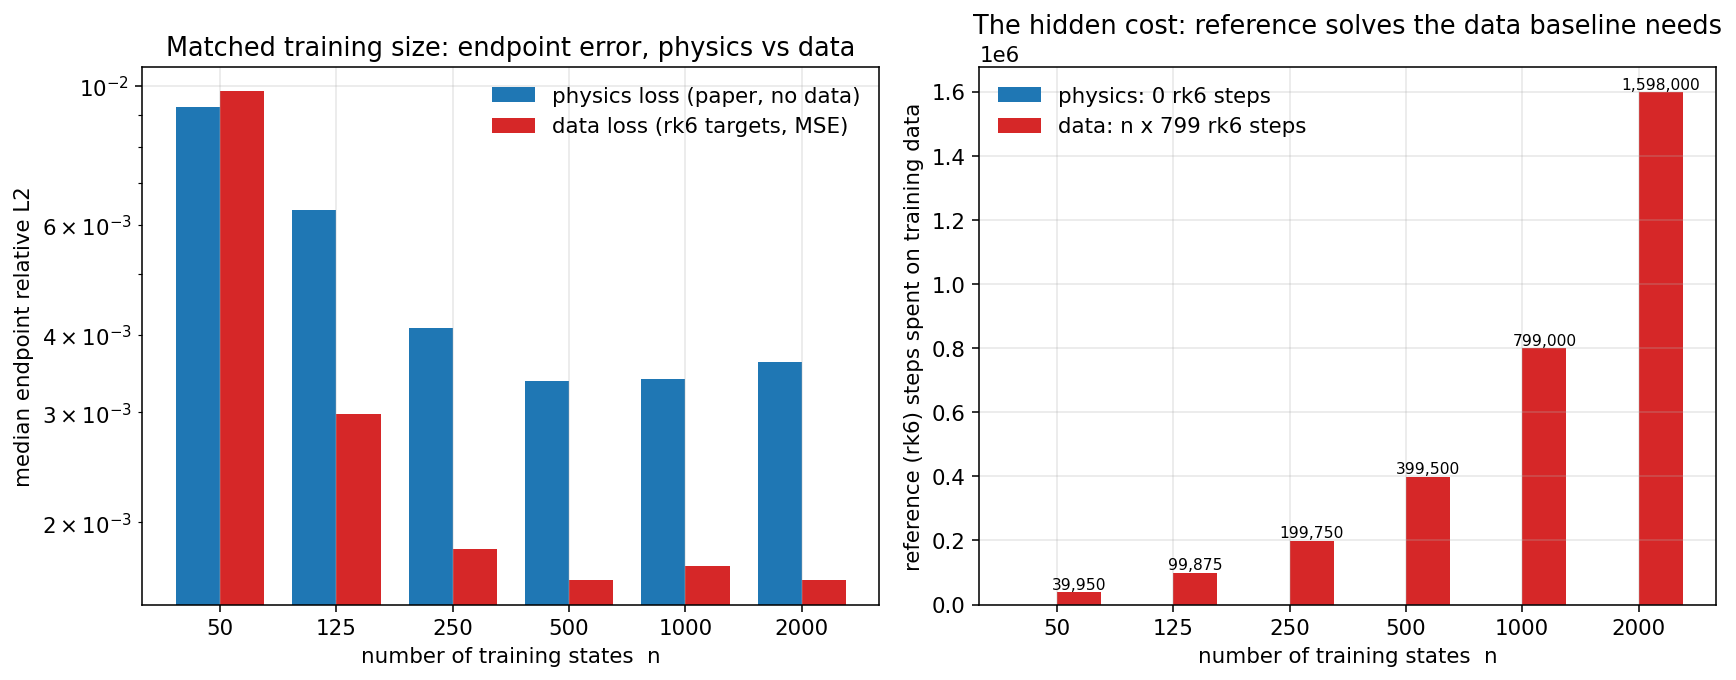
\includegraphics[width=\linewidth]{fig_data_baseline.png}
  \caption{Accuracy against training-set size for the matched pair (left)
  and the hidden cost of the data arm (right): the physics arm's
  reference-data bill is zero everywhere.}
  \label{fig:data-baseline}
\end{figure}

% ===========================================================================
\section{Discussion}
\label{sec:discussion}

\paragraph{Relation to the source work.}
Where the regimes overlap, the reproduction agrees: on sub-period
horizons, the same regime as the source work's continuous-time solution
demonstrations (which span at most one time unit or $\pi/2$), the
transcription meets or betters the reported accuracy of a few $10^{-4}$ to
$2\times10^{-3}$. Where the source work stops, the measurements sharpen it
in three ways. First, it frames the continuous-time formulation's principal
limitation as the \emph{cost} of collocation in higher dimensions. On this
problem the collocation budget is trivial and fully paid
(Section~\ref{sec:collocation}), was then varied 64-fold and
placement-optimised to no effect (Sections~\ref{sec:density}
and~\ref{sec:placement}), and the formulation fails anyway, through
optimisation collapse onto zero-residual impostor solutions with a
converged loss. This is a direct counterexample to its sufficiency claim,
backed by 733 runs rather than 15, so cost is not the binding limitation
on long horizons even in one dimension. Second, on the discrete-time side
the source work attributes its Allen--Cahn error to network capacity, and
its appendix tables already contain a visible error floor (its $q$-sweep
at $\Delta t = 0.8$ flattens at $7\times10^{-4}$--$1.2\times10^{-3}$ from
$q = 16$ to $q = 500$); what it lacks is the exactly solved scheme on the
same states and metric, which is what turns a plateau in a table into an
attribution (scheme-limited at $q = 2$, network-limited from $q = 4$).
The 135-run architecture sweep then goes one step further than the source
work's capacity attribution: the loss--error rank correlation of $+0.974$
makes the floor an optimisation floor, which no network size
fixes. Third, its stage-count prescription (choose $q$ so that the
theoretical $\mathcal{O}(\Delta t^{2q})$ truncation reaches machine
precision, giving $q \approx 81$ at $\Delta t = 0.8$) is far past the
point of usefulness once the optimisation binds: at $q = 8$ the scheme
already sits five orders of magnitude below the floor. Finally, the
source work's implied single-giant-step reading (``resolve the entire
spatio-temporal solution in a single step'') does not transfer
unconditionally: on this system the nonlinear stage equations stop being
reliably solvable near a full-period step, a solvability caveat, distinct
from stability, that the source work does not discuss, and at the
largest feasible step chaining beats the one-shot mode by a factor 10
(Section~\ref{sec:disc-routes}).

\paragraph{Relation to the causal-weighting literature.}
The rescue behaves exactly as its authors report~\cite{wang2024causal}: it
fixes the pathology it targets, the simultaneous fitting of all times, at
a training cost that grows quickly with the domain, and their own guidance
that causal weighting complements rather than replaces
time-marching~\cite{wang2023expert} is precisely what
Sections~\ref{sec:causal} and~\ref{sec:disc-routes} measure from the two
sides. A fixed look-back window (weighting each point only by the residual
of the preceding period) was considered and rejected without an
experiment: a fit that jumps once and then follows a different genuine
solution of the equation has zero residual inside every window older than
the jump, so windowing re-admits silent impostors. The whole-history
integral in Eq.~\eqref{eq:causal} is the quarantine that keeps unreached
territory asleep, and the same integral is what makes the annealing bar
tighten with horizon. The density study adds one new fact to this
literature: the causal certificate itself has a density floor
(approximately 20 points per unit time here) below which certified
arrival is actively misleading (Section~\ref{sec:density}). The failure
modes measured here sit within the broader literature on PINN optimisation
pathologies~\cite{wang2021gradient,krishnapriyan2021}, and sharpen it with
an unusual amount of instrumentation per failure.

\paragraph{The recurring lesson.}
The equation alone admits many solutions, and any stretch of the domain the
loss cannot see is eventually exploited by the optimiser: late times in the
plain formulation, the unsampled gap after $t = 0$ in the causally weighted
one, the space between any two collocation points in the extended-budget
runs. Each fix closed one loophole and exposed the next, at increasing
cost. The resource axes are now all measured null, so what remains is
geometry: success is a start-dependent probability falling toward the
repelling equilibrium. Two corollaries deserve emphasis. Phase-space
agreement is necessary but never sufficient: an orbit can lie exactly on
the limit cycle and be order-one wrong in time
(Figure~\ref{fig:extended-phase}). And in every failure the training loss
was small: the verdict must always come from the error against a trusted
reference at points the training never saw, and never from the loss. The
discrete-time formulation removes the disease rather than treating it:
every output is tied to a known state through the algebra of the step, so
a spurious solution has nowhere to live. It is no coincidence that this is
also the only formulation here whose loss honestly predicts its error, all
the way to a rank correlation of $+0.974$ across 135 architectures.

% ===========================================================================
\section{Future work}
\label{sec:future}

Four studies follow naturally from these measurements; I list them in the
order I expect them to pay off.

\begin{itemize}
  \item \textbf{Attribution of the optimisation floor.} The 135-run sweep
  rules out capacity; what it does not yet separate is optimiser dynamics
  from the loss landscape: whether a different optimiser class, training
  schedule, or curriculum over the training region moves the
  $3.6\times10^{-3}$ floor at fixed architecture.
  \item \textbf{The annealing schedule.} The measured tightening of the
  causal wake-up criterion with horizon suggests the variant
  $\varepsilon \propto 1/T$, which directly targets the whole-history
  integral's growth; the placement and density studies fix everything
  needed to test it in isolation.
  \item \textbf{Inverse problems.} The source work's data-driven discovery
  setting, recovering the damping parameter $\mu$ from noisy
  observations, has a natural discrete-time variant that reuses exactly
  the trained reconstructions with $\mu$ as a free parameter.
  \item \textbf{Learned quadrature.} A variant in which the network
  predicts the step's weights rather than its states, for which the
  fine-grained single-step reference built for this study provides the
  supervision.
\end{itemize}

% ===========================================================================
\section{Conclusion}
\label{sec:conclusion}

On a fully controlled nonlinear oscillator with a reference solution
trusted to $10^{-13}$, the continuous-time PINN formulation is excellent
below one period of the limit cycle and fails structurally beyond it,
collapsing onto zero-residual spurious solutions while its training loss
converges. The failure survives every resource offered to it: ample
collocation, a four-fold optimisation budget, 25 network architectures at
600 runs, a 64-fold density range, and targeted re-placement of the
collocation points. The strongest loss-level remedy postpones it by one
period at a cost that grows faster than linearly, and what finally orders
the outcomes is the geometry of the starting state relative to the
repelling equilibrium: success at two periods is a 12.7\% gamble at the
1\% error bar, and at four periods no run of 150 wins it. The
discrete-time formulation, generalised into a reusable flow map over
starting states, inherits none of this. Its supervision is anchored to a
known state by the algebra of an implicit Runge--Kutta step, its training
loss is an honest proxy for its error, and its accuracy is cleanly
attributable: scheme-limited at two stages, floored at $3.6\times10^{-3}$
from four by the optimisation rather than by capacity. Its long-horizon
quality, decided by the training seed, is measurable on a validation
chain and fixed by a simple selection protocol. The selected network,
chained without retraining, carries 108 held-out starting states through
six periods at $2.0\times10^{-3}$ relative error, holds flat to thirty
periods on fresh starts, and beats the single-giant-step reading of the
source work by a factor 10 at the largest step the nonlinear algebra
allows; a matched data-supervised twin shows the physics costs a factor
2.1 in accuracy against perfect labels and zero reference data in
exchange. For initial-value problems on long horizons, the measured
advantage lies with formulations that re-anchor the physics on known
states step by step, and the continuous-time formulation's known
weaknesses understate the case: the binding failure is the optimiser's
freedom to satisfy the equation on the wrong solution, rather than the
cost of enforcing it.

% ---------------------------------------------------------------------------
\section*{Data availability}

All training scripts, saved results, and the notebooks that generate every
figure and number in this paper are available at
\url{https://github.com/GeorgeWilliam1999/Van_Der_Pole}. All experiments
are seeded and reproduce deterministically; the reference solution and its
verification are included.

% \section*{Acknowledgements}
% TODO before submission.

\bibliographystyle{unsrtnat}
\bibliography{references}

\end{document}
